\documentclass[11pt, a4paper, oneside]{book}

\usepackage{fancyhdr}
\pagestyle{fancy}
\fancyhf{}

\usepackage[english]{babel}
\usepackage{graphicx}
\usepackage[colorlinks,hyperindex,plainpages=false,breaklinks]{hyperref}
\usepackage{amssymb}
\usepackage{wasysym} 
\usepackage{wrapfig}
\usepackage{enumerate}
\usepackage{placeins} % Necessary for \FloatBarrier
\usepackage{subfig}   % Necessary for subfloat (images next to each other)
\usepackage{color}
\usepackage[usenames,dvipsnames,svgnames]{xcolor}
\usepackage{listings}

\definecolor{codelightgray}{rgb}{0.87,0.87,0.87}

\hypersetup{colorlinks=true,% 
	linkcolor=black,%
	citecolor=red,%
	filecolor=blue,% 
	menucolor=black,% 
	pagecolor=black,%
	urlcolor=black
}

\lstset{language=,
    keywordstyle=\color{blue},
    basicstyle=\scriptsize\ttfamily,
    showstringspaces=false,
    backgroundcolor=\color{codelightgray},
    morekeywords={SELECT,FROM,WHERE,AND,OR,EClass}
}

\setcounter{tocdepth}{1}

\setlength{\parindent}{0pt} 
\setlength{\parskip}{0.3cm}

% Remove section numbers 0.1, 0.2 ..
\renewcommand{\thesection}{\arabic{section}} 

\graphicspath{%
{../../06_miscellaneous/commonFiles/}% Title image and memBox illustration
{../01_LeitnersBoxReviewed/lbrImages/}%
{../02_transformationsExplained/teImages/}%
{../03_removeCard/splashImages/}{../03_removeCard/GUIImages/}{../03_removeCard/visRemImages/}{../03_removeCard/texRemImages/}%
{../04_checkCard/splashImages/}{../04_checkCard/visCheImages/}{../04_checkCard/texCheImages/}%
{../05_LLBGuiExtended/}%
{../06_emptyPartition/}{../06_emptyPartition/visEPImages/}{../06_emptyPartition/texEPImages/}%
{../07_invertCard/}{../07_invertCard/visICImages/}{../07_invertCard/texICImages/}%
{../08_growBox/}{../08_growBox/visGBImages/}{../08_growBox/texGBImages/}%
{../09_conditionalBranching/}{../09_conditionalBranching/visCBImages/}{../09_conditionalBranching/texCBImages/}%
{../10_stringRep/}{../10_stringRep/visSRImages/}{../10_stringRep/texSRImages/}%
{../11_fastCards/}{../11_fastCards/visFCImages/}{../11_fastCards/texFCImages/}%
}

% --- HEADER FUNCTIONS ----------------------------------------------------------------------------------------------------------------------------------------
% Default plain header; turn off all lines and colors; turn on page numbers for all
\newcommand{\noHeader}{
	\fancyfoot{}
 	\fancyhead[R]{\thepage}
	\fancyhead[L]{}
	\renewcommand{\headrulewidth}{0pt}
}

% Common instruction Header; Black
\newcommand{\genHeader}{
	\fancyfoot{}
	\fancyhead[L]{}
	\renewcommand{\headrulewidth}{1.5pt}
 	\renewcommand{\headrule}{\hbox to\headwidth{%
  		\color{Black}\leaders\hrule height \headrulewidth\hfill}}
}

% Visual instructions; Red header
\newcommand{\visHeader}{
	\fancyfoot{}
	\fancyhead[L]{\color{RedOrange}\tiny \bf VISUAL}
	\renewcommand{\headrulewidth}{1.5pt}
	\renewcommand{\headrule}{\hbox to\headwidth{%
  		\color{RedOrange}\leaders\hrule height \headrulewidth\hfill}}
}

% Text instructions; Blue header
\newcommand{\texHeader}{
	\fancyfoot{}
	\fancyhead[L]{\color{CornflowerBlue}\tiny \bf TEXTUAL}
	\renewcommand{\headrulewidth}{1.5pt}
	\renewcommand{\headrule}{\hbox to\headwidth{%
  		\color{CornflowerBlue}\leaders\hrule height \headrulewidth\hfill}}
}

% --- FORMATTING COMMANDS --------------------------------------------------------------------------------------------------------------------------------------
% 'Next..' jump links (bottom right)
\newcommand{\jumpSingle}[1]{
\fancyfoot[OR]{$\triangleright$ \hyperlink{#1}{\texttt{Next}}}
}

\newcommand{\jumpDual}[2]{
\fancyfoot[RO]{ $\triangleright$ \hyperlink{#1}{\texttt{Next [visual]\hspace{0.2cm}}}%
 \\ $\triangleright$ \hyperlink{#2}{\texttt{Next [textual]}}}
}

% These words should appear in the glossary
\newcommand{\define}[1]{\marginpar{\small\emph{#1}}}

% Textual syntax EBNF statement format
\newcommand{\syntax}[1]{ \begin{quote} \small \texttt{#1} \end{quote}}

% Required time for part (Should appear on introduction page)
\newcommand{\requiredTime}[1]{ {\scriptsize \texttt{Approximate time to complete: #1} } }

% TODO: update download link (RE: part descriptions) ----------------------------------------------------------------------------------------------------------
\newcommand{\dlPartZero}{\url{www.emoflon.org}}

%--------------------------------------------------------------------------------------------------------
\def\partTitle{Part III: Story Driven Modelling}
\title{
\flushright
{\LARGE\bfseries An Introduction to Metamodelling\\
and Graph Transformations}
\noindent\rule[-1ex]{\textwidth}{5pt}\\[2.5ex]
\hfill\emph{\LARGE\bfseries with eMoflon}
\flushleft
{\small Version 2.1}
\flushright

\includegraphics[width=0.85\textwidth]{pics/eMoflon3} 
}

\date{}  
\author{} 
% Version 0.1:	initial release
% version 0.2:	minor spelling/formatting edits, etc.
% -------------------------------------------------------------------------------------------------------------------------------------------------------------

\begin{document}

\frontmatter
\noHeader

{\let\newpage\relax\maketitle}

\begin{small} 
Copyright \copyright~2011--\the\year{} Real-Time Systems Lab, TU Darmstadt.
Anthony Anjorin, Erika Burdon, Frederik Deckwerth, Roland Kluge, Marius Lauder,
Erhan Leblebici, Daniel T\"ogel, David Marx, Lars Patzina, Sven Patzina, Alexander Schleich, Sascha Edwin Zander, Jerome Reinl\"ander, Martin Wieber, and contributors.
All rights reserved.

This document is free; you can redistribute it and/or modify it under the terms of the GNU Free Documentation License as published by the Free Software Foundation; either version 1.3 of the License, or (at your option) any later version.
Please visit \href{http://www.gnu.org/copyleft/fdl.html}{http://www.gnu.org/copyleft/fdl.html} to find the full text of the license.
 
% TODO Remove this?? It can be found easily online .. (we can even offer it on
% the download page) For your convenience, this document includes a copy of the \emph{GNU General Public License} starting from page~\pageref{chap:gpl}.
  
For further information contact us at \eMoflonContact.
  
\vskip3cm
\textit{The eMoflon team}\\
Darmstadt, Germany (\monthword{\month} \the\year)
\end{small}
\let\cleardoublepage\clearpage

\tableofcontents

% Store page counter
\newcounter{romanpages}
\setcounter{romanpages}{\value{page}}

\mainmatter

% Main content for this Part; handles all inputs
\part{Story Driven Modelling}
\label{chap:sdm}
\newpage

\genHeader
\requiredTime{2 h}

Welcome to Part III, an introduction to unidirectional model transformations via programmed graph transformations using Story Driven Modeling (SDM).
SDMs focus on concrete implementations, so we plan to implement the methods signatures declared in the abstract syntax. It other words, this is where you'll
build your metamodel's dynamic semantics! Don't let the sheer size of this part frighten you off. We have included deep, thorough explanations (with an ample
number of figures) to ensure the concepts are crystal clear - it's really not that bad.

In Part II, we learned that we can implement methods in a straightforward manner with injections and Java code, so why bother with SDMs? 

Overall, SDMs are a simpler, alternate way of implementing methods. Rather than building verbose Java code yourself, you can model each action individually then
generate the corresponding code to implement it. With the visual syntax, the advantage is obvious. You'll be able to use familiar, easy-to-understand UML
activity diagrams to establish your methods. Texually, SDMs extend the Objected Oriented Paradigm by separating all classes, references, and activities into
different files, folders, and patterns.

If you're just joining us, read the next section for a brief overview of our running example so far, and how to download some files that will help you get
started right away. If you're continuing from Part II, click the link below to continue with your constructed learning box metamodel.

\begin{center}\texttt{$\triangleright$ \hyperlink{explanation}{Continue from Part II\ldots}}\end{center}


\section{Leitner's learning box reviewed}

\emph{Leitner's learning box}\footnote{\href{http://en.wikipedia.org/wiki/Leitner\_system}{http://en.wikipedia.org/wiki/Leitner\_system}} is a simple, but
ingenious little contraption to support the tedious process of memorization, especially prominent when trying to learn, for example, a new language. As depicted in
Fig.~\ref{fig:membox_depiction}, this box consists of a series of partitions with a strict set of rules. The contents to be memorized are written on little cards and placed in the first container. Every
time the user correctly answers a card, that card is promoted to the next partition. Once it reaches the final partition, it can be considered memorized, and
no longer needs to be practiced. Every time the user incorrectly answers a card however, it is returned to the original starting partition, and the
learning process is restarted.

\begin{figure}[htbp]
	\centering
  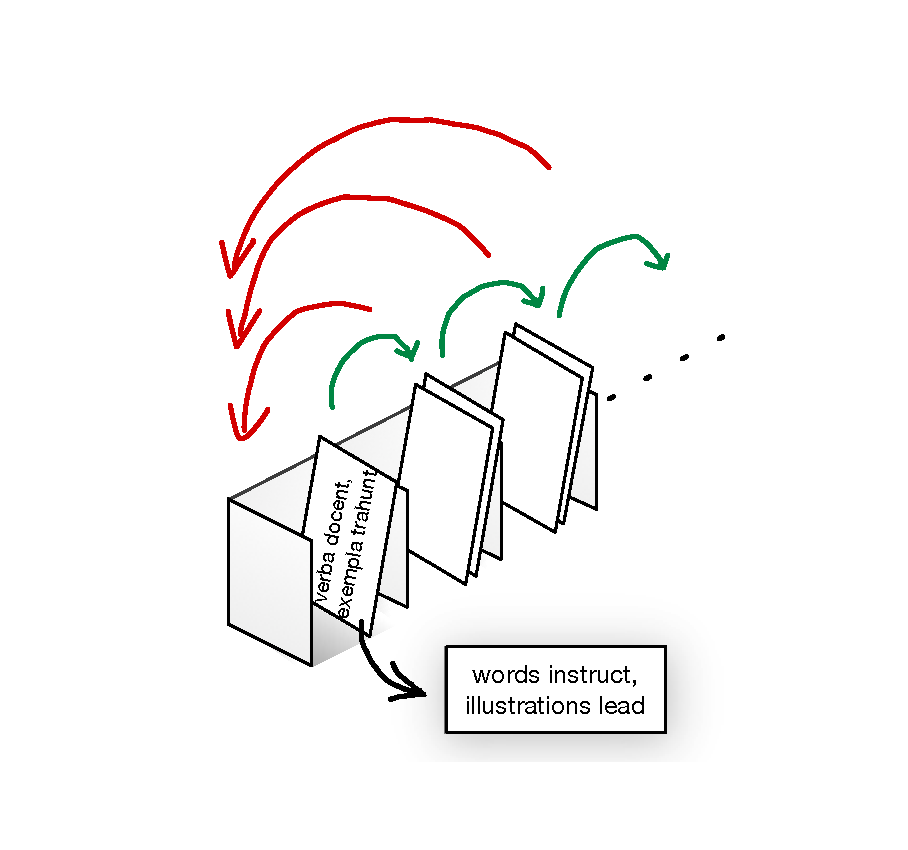
\includegraphics[width=0.4\textwidth]{membox_illustration.pdf}
	\caption{Static Structure of a Leitner's Learning Box}
	\label{fig:membox_depiction}
\end{figure}

For a more detailed overview of the box and our goals, we recommend you read the introduction to Part II. But for now, enough discussion!

\begin{itemize}

\item[$\blacktriangleright$] To get started, press the \texttt{new} button and navigate to ``Examples/eMoflon Handbook Examples/''
(Fig.~\ref{fig:downloadWizard}).

\begin{figure}[htbp]
	\centering
  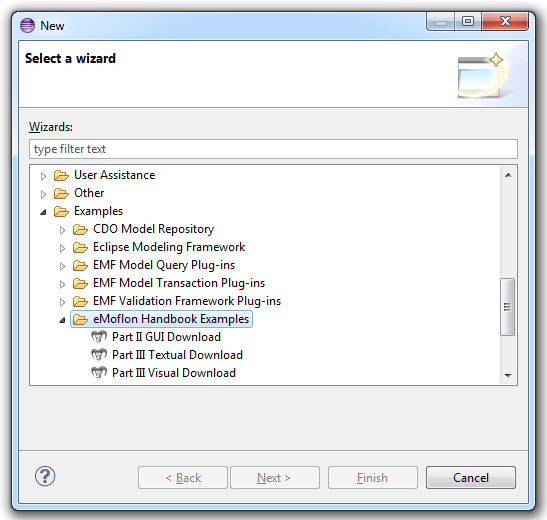
\includegraphics[width=0.75\textwidth]{eclipse_downloadWizard}
	\caption{Download a file set to get started}
	\label{fig:downloadWizard}
\end{figure}

\item[$\blacktriangleright$] Download the file package of the eMolfon specification type you'd like to learn. Remember, with the visual syntax, you'll be
using an external modeling program to craft your metamodel diagrams, then exporting the data to Eclipse for generation. With textual, you'll be working entirely
within the Eclipse IDE in the eMolfon perspective.

\newpage

\vspace*{0.5cm}

\item[$\blacktriangleright$] If your package explorer does not resemble ours in Fig.~\ref{fig:workingSets} with at least two distinct nodes, select the
small, downward facing arrow in the corner of the module window. Choose ``Working Sets'' as your ``Top Level Elements''. We use these to structure the workspace
in Eclipse.

\vspace{0.75cm}

\end{itemize}

\begin{figure}[htbp]
	\centering
  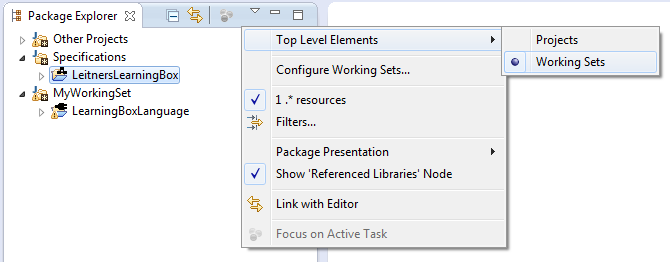
\includegraphics[width=0.9\textwidth]{eclipse_workingSets}
	\caption{Setting your Package Explorer \update}
	\label{fig:workingSets}
\end{figure}

The ``MyWorkingSet" node contains \texttt{Learn\-ing\-Box\-Lang\-uage}, which in turn contains all the code generated from your metamodel. The metamodel itself
is found in \texttt{Leit\-ners\-Learn\-ing\-Box} under ``Specifications''. The visual metamodel is a single \texttt{.eap} file, while the textual metamodel is
contained within an explicit project structure. 

These sets are not included under same node due to being different \emph{nature}s, or project types. \texttt{Learning\-Box\-Language} is your
\emph{repository project}, the Eclipse classification of a normal Java project.\footnote{For details on the project setup, review Part I, sections 4 and 5} 

\begin{itemize}

\item[$\blacktriangleright$] Inspect the files in both nodes until you feel comfortable with what you'll be working with. In particular, look at the files found
under ``gen." Each Java file has a corresponding \texttt{.impl} file, where all actionable code (such as method implementations) will be placed.\footnote{For
specific details on their contents, refer to Part II, section 5} 

\item[$\blacktriangleright$] Be sure to also review the ecore model under ``LearningBoxLanguage/model/'' and the dynamic instance found in ``instances.'' While
you can make and customize your own instance,\footnote{To learn how to make your own instance model, review Part II, section 4} we have included a small sample
in your download to help you get started.

\end{itemize}

Well, that's it! A quick review, paired with a fine download makes an excellent appetizer to SDMs. Let's get started.

\newpage
\hypertarget{explanation}{}
\section{Transformations explained}
\genHeader

The core idea when modeling behaviour is to regard dynamic aspects of a system (let's call this a model from now on) as bringing about a change of state.
This means a model in state $S$ can evolve to state $S^*$ via a transformation $\Delta: S \stackrel{\Delta}{\rightarrow}S^*$. In this light, dynamic or
behavioural aspects of a model are synonymous with \emph{model transformations}, and the dynamic semantics of a language equates simply to a suitable set of
model transformations. This approach is once again quite similar to the object oriented (OO) paradigm, where objects have a state, and can \emph{do} things via
methods that manipulate their state.

So how do we \emph{model} model transformations?  There are quite a few possibilities. We could employ a suitably concise imperative programming language in
which we simply say how the system morphs in a step-by-step manner. There actually exist quite a few very successful languages and tools in this direction. But
isn't this almost like just programming directly in Java? There's got to be a better way! 

From the relatively mature field of graph grammars and graph transformations, we take a \emph{declarative} and \emph{rule-based} approach. Declarative in this
context means that we do not want to specify exactly how, and in what order, changes to the model must be carried out to achieve a transformation. We just want
to say under what conditions the transformation can be executed (precondition), and the state of the model after executing the transformation (postcondition).
The actual task of going from precondition to postcondition should be taken over by a transformation engine, where all related details are basically regarded as
a black box.

So, inspired by string grammars and this new, refined idea of a model transformation (which is of the form $(pre, post)$), let's call this black box
transformation a \emph{rule}. It follows that the precondition is the left-hand side of the rule, $L$, and the postcondition is the right-hand side, $R$.

A rule, $r: (L,R)$, can be \emph{applied} to a model (a typed graph) $G$ by:
\begin{enumerate}
  \item \emph{Finding} an occurrence of the precondition $L$ in $G$ via a \emph{match}, $m$
  
  \item \emph{Cutting} out or $Destroying$ $(L\setminus R)$, i.e., the elements that are present in the precondition but not in the postcondition are deleted
  from $G$ to form  $(G\setminus Destroy)$
  
  \item \emph{Pasting} or $Creating$ $(R\setminus L)$, i.e., new elements that are present in the postcondition but not in the precondition and are to be created
  in the hole left in $(G\setminus Destroy)$ to form a new graph, $H = (G\setminus Destroy) \cup Create$ (\Cref{fig:rule_application}). 
  
  \end{enumerate}

\vspace{0.5cm}

\begin{figure}[htp]
\begin{center}
  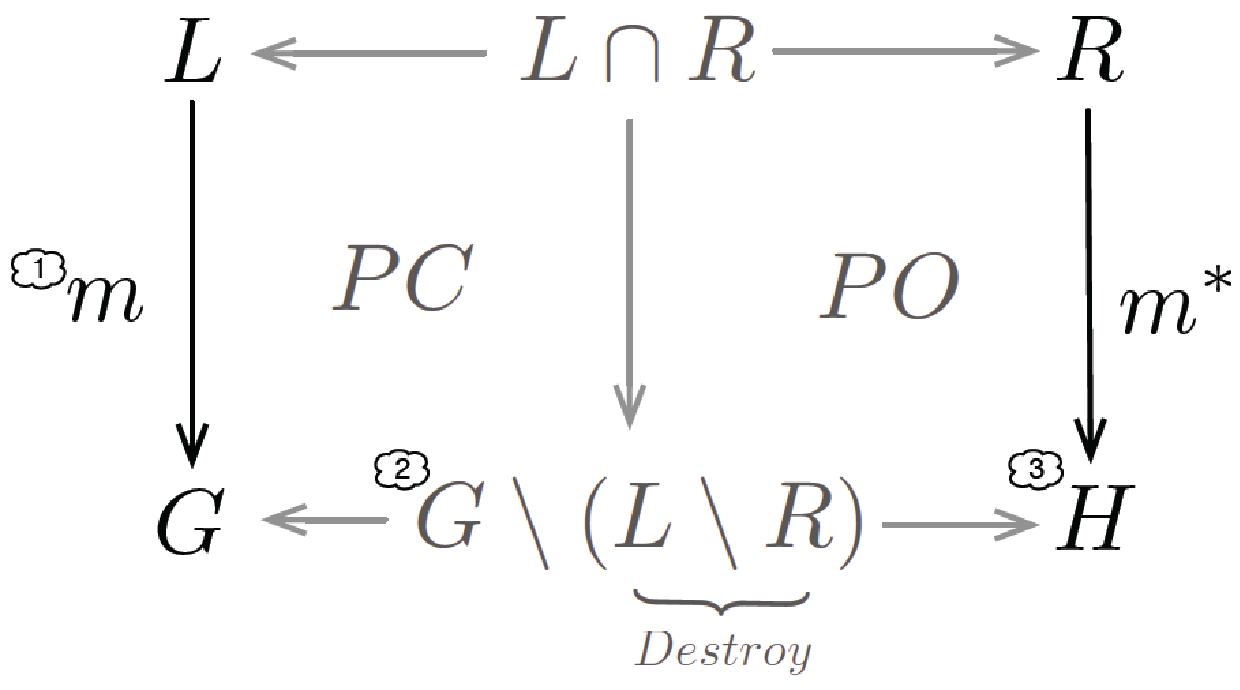
\includegraphics[width=0.8\textwidth]{../../org.moflon.doc.handbook.03_storyDiagrams/02_transformationsExplained/teImages/rule_application}
  \caption[]{Applying a rule $r: (L,R)$ to $G$ to yield $H$} 
  \label{fig:rule_application}
\end{center}
\end{figure}

\vspace{0.5cm}

Let's review this application. 

(1) is determined by a process called \emph{graph pattern matching}\define{Pattern Matching} i.e., finding an occurrence or
\emph{match} of the precondition or \emph{pattern} in the model $G$.

(2) is determined by building a \emph{push-out complement} $PC = (G\setminus Destroy)$, such that $L\cup PC = G$.

(3) is determined by building a \emph{push-out} $PO = H$, so that $(G\setminus Destroy) \cup R = H$.

A push-out (complement) is a generalised union (subtraction) defined on typed graphs. Since we are dealing with graphs, it is not such a trivial task to define
(1) -- (3) in precise terms, with conditions for when a rule can or cannot be applied. A substantial amount of theory already exists to satisfy this goal.

Since this black box formalisation involves two push-outs - one when cutting $Destroy := (L\setminus R)$ from $G$ to yield $(G\setminus Destroy)$ (deletion),
and one when inserting $Create := (R\setminus L)$ in $(G\setminus Destroy)$ to yield $H$ (creation) - this construction is referred to as a \emph{double
push-out}. We won't go into further details in this handbook, but the interested reader can refer to \cite{EEPT06} for the exciting details.

Now that we know what rules are, let's take a look at a simple example for our learning box. What would a rule application look like for moving a card from
one partition to the next? \Cref{fig:rule_example} depicts this $moveCard$ rule.
  
\begin{figure}[htp]
\begin{center}
  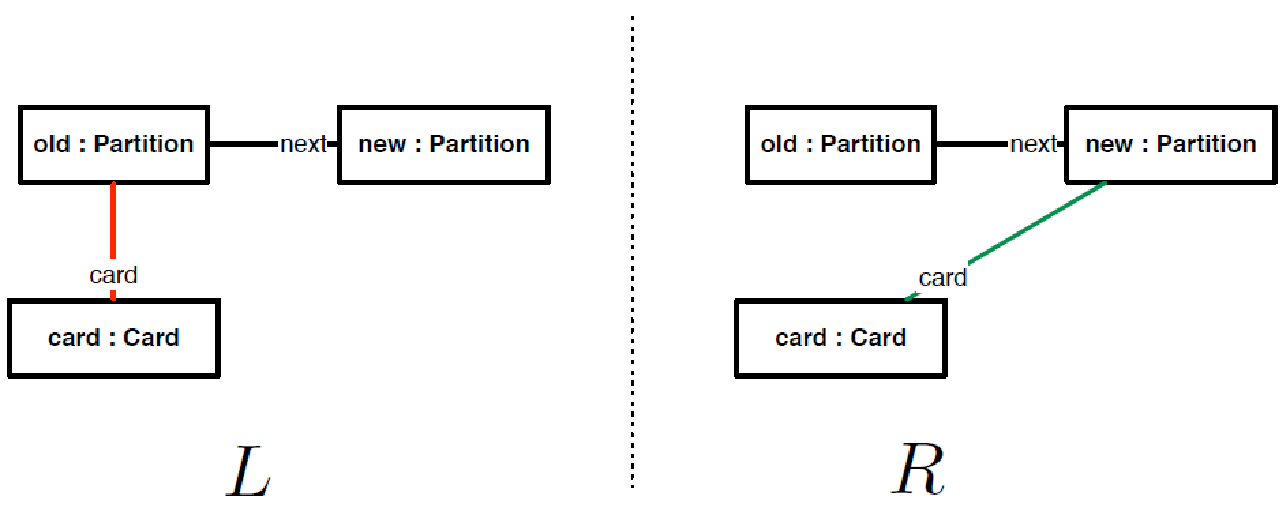
\includegraphics[width=1\textwidth]{../../org.moflon.doc.handbook.03_storyDiagrams/02_transformationsExplained/teImages/rule_example}
  \caption[]{$moveCard$ as a graph transformation rule}	
  \label{fig:rule_example}
\end{center}
\end{figure}


As already indicated by the colours used for $moveCard$, we employ a compact representation of rules formed by merging $(L,R)$ into a single \emph{story
pattern}\define{Story Pattern} composed of  $Destroy := (L\setminus R)$ in red, $Retain :=  L\cap R$ in black, and $Create := (R\setminus L)$ in green
(\Cref{fig:rule_compact}).

\begin{figure}[htp]
\begin{center}
  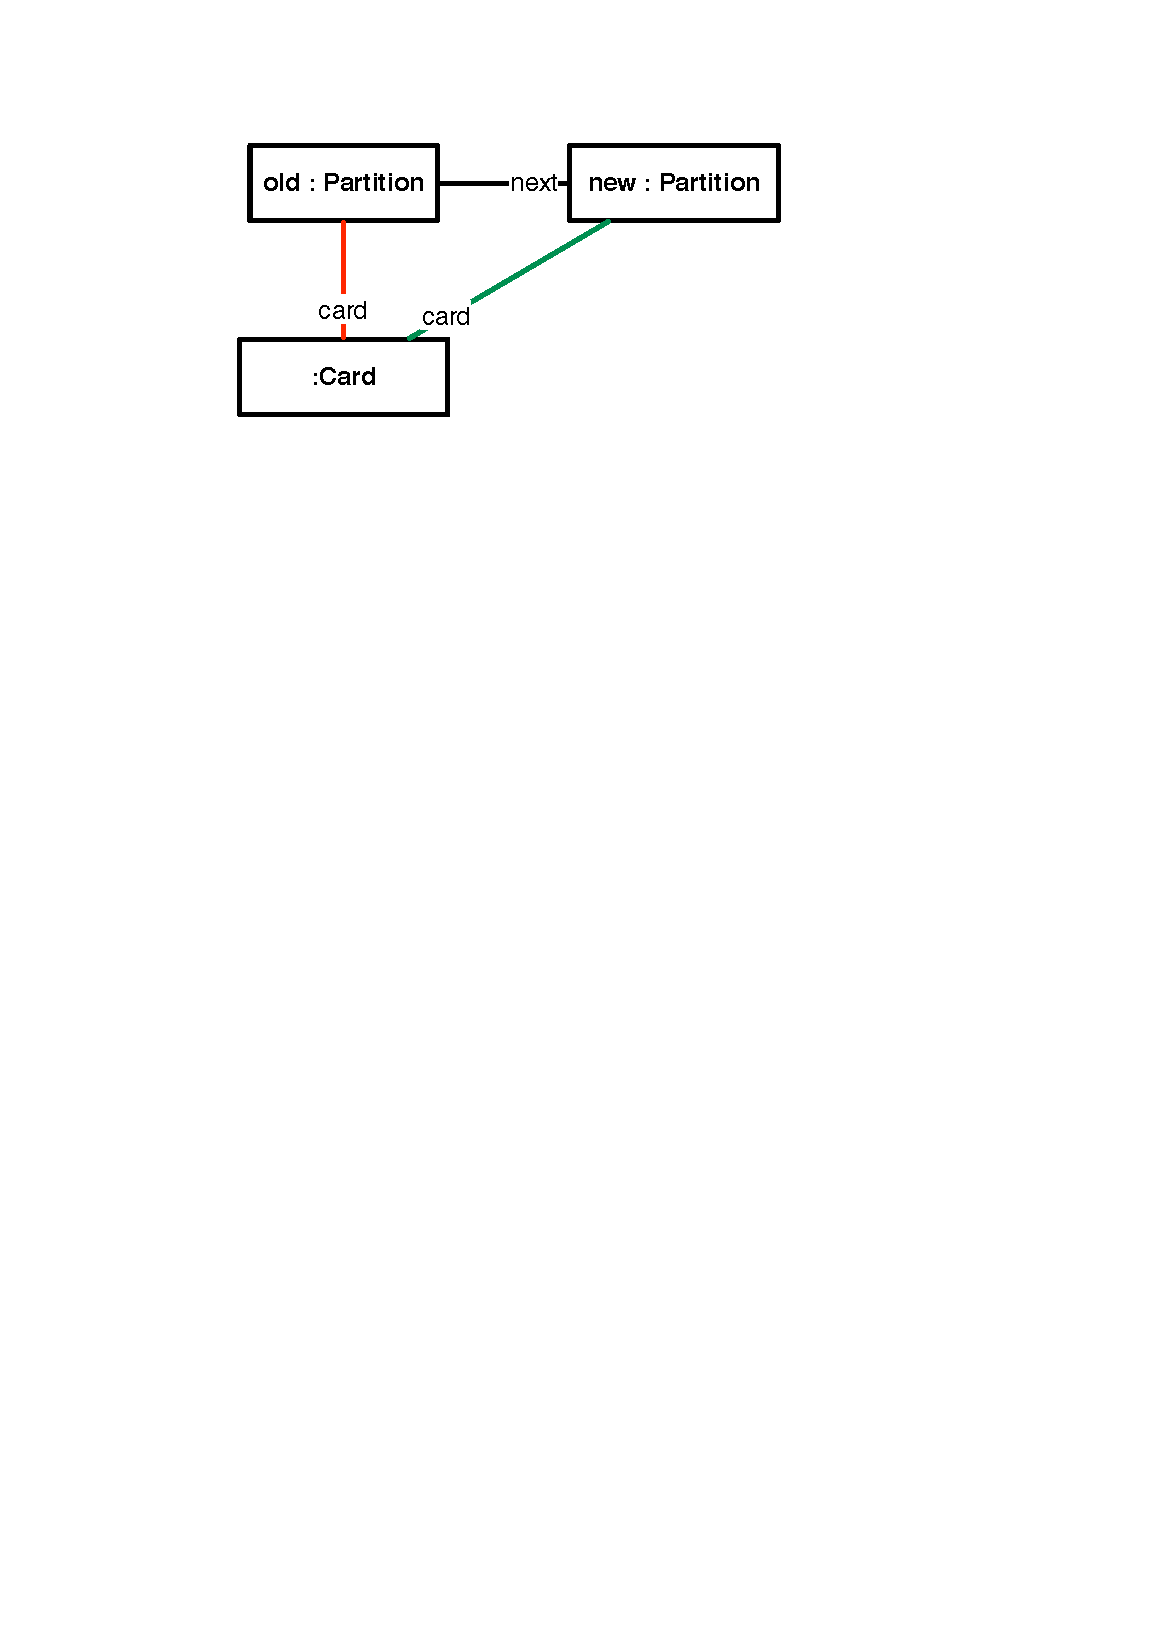
\includegraphics[width=0.45\textwidth]{../../org.moflon.doc.handbook.03_storyDiagrams/02_transformationsExplained/teImages/rule_compact}
  \caption[]{Compact representation of $moveCard$ as a single \emph{story pattern}}
  \label{fig:rule_compact}
\end{center}
\end{figure}

As we shall see in a moment, this  representation is quite intuitive, as one can just forget the details of rule application and think in terms of what is to be
deleted, retained, and created. We can therefore apply $moveCard$ to a learning box in terms of steps (1) -- (3), as depicted in \Cref{fig:rule_app_example}.

Despite being able to merge rules together to form one story pattern, the individual rules still have to be applied in a suitable sequence to realise complex
model transformations consisting of many steps! This can be specified with simplified activity diagrams, where every \emph{activity node}\define{Activity Node}
or \emph{story node} contains a single \emph{story pattern}, and are combined with the usual imperative constructs to form a control flow structure. The entire
transformation can therefore be viewed as two separate layers: an imperative layer to define the top-level control flow via activities (i.e., if/else
statements, loops, etc.), and a pattern layer where each story pattern specifies (via a graph transformation rule) how the model is to be manipulated.

\pagebreak

\vspace*{2cm}

\begin{figure}[htp] 
\begin{center}
  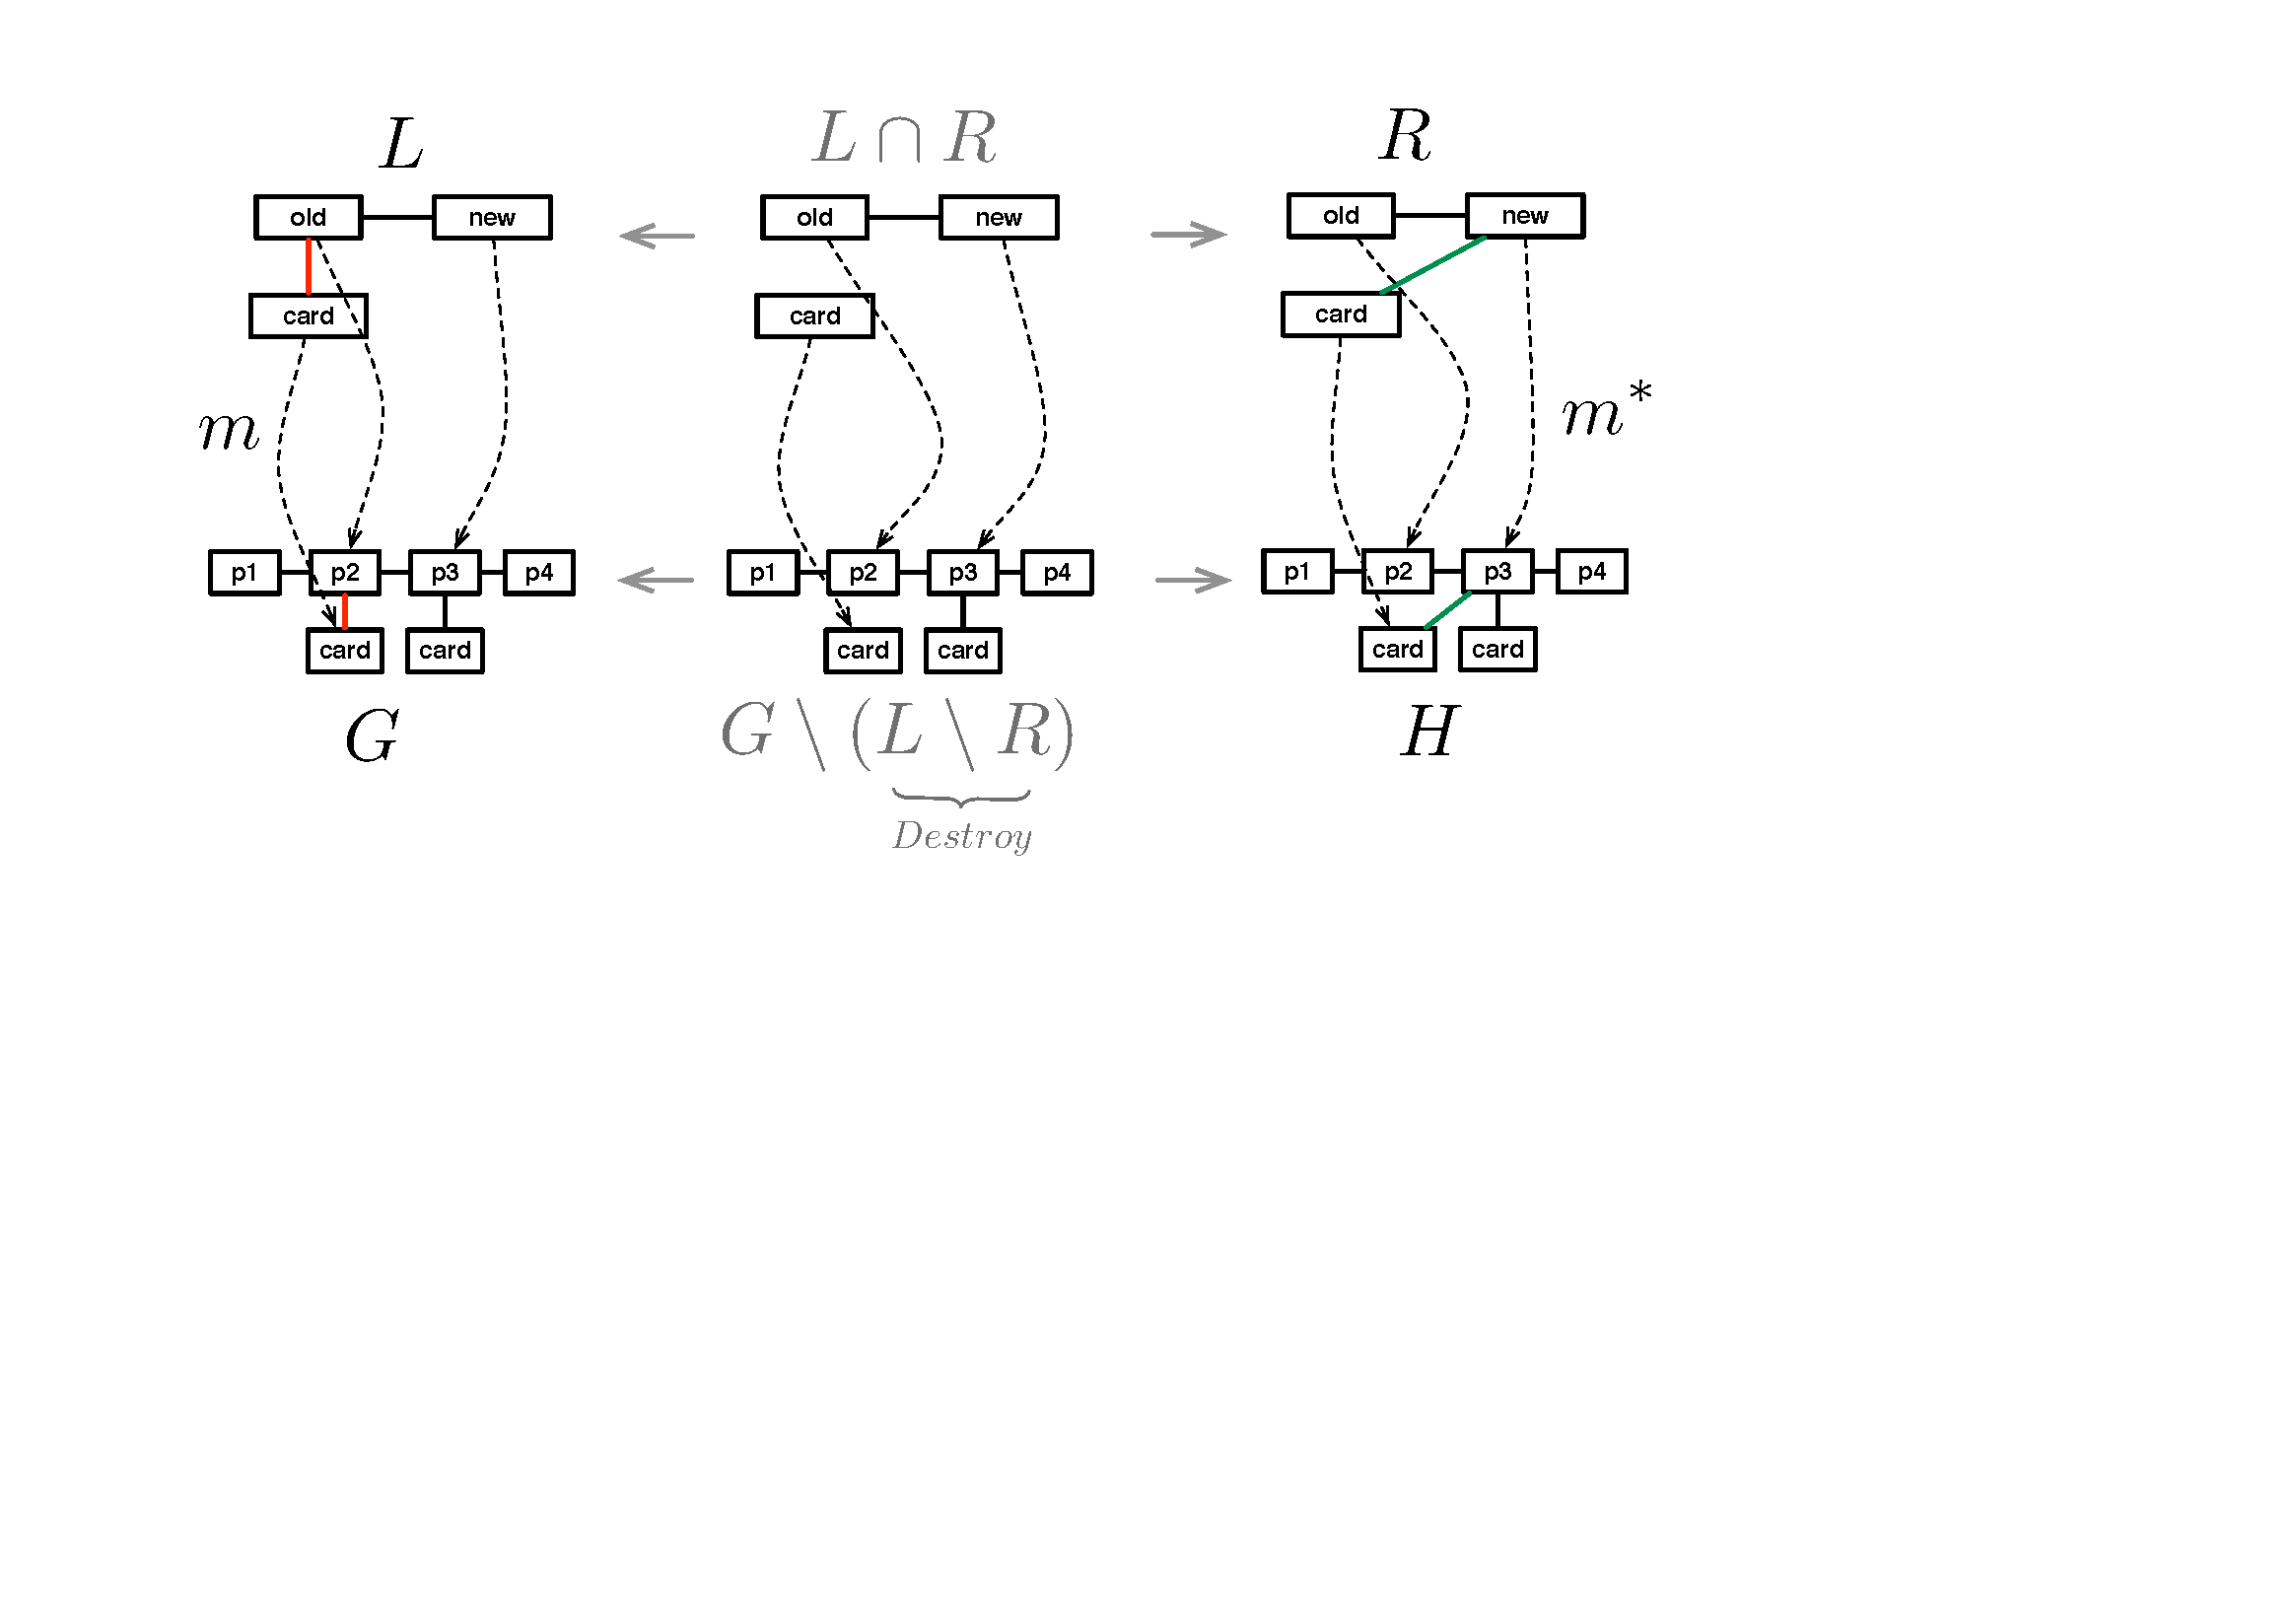
\includegraphics[width=1\textwidth]{../../org.moflon.doc.handbook.03_storyDiagrams/02_transformationsExplained/teImages/rule_app_example}
  \caption[]{Applying $moveCard$ to a learning box}
  \label{fig:rule_app_example}
\end{center}
\end{figure}

\vspace*{1cm}

Enough theory! Grab your mouse and let's get cracking with SDMs\ldots


\newpage
\genHeader
\section{Removing a card}
\hypertarget{sec:remCard}{}

Since we're just getting started with SDMs,\footnote{As you may have already noticed, we use ``SDM'' or ``Story Diagrams" interchangeably to mean both our graph
transformation language \emph{or} a concrete transformation used to implement a method, consisting of an activity with activity nodes containing story
patterns.} let's re-implement the method previously specified directly in Java as an injection.\footnote{Refer to Part II, Section 6} The goal of this method
is to remove a single card from its current partition, which can be done by destroying the link between the two items (\Cref{fig:goal_removeCard}).

\vspace{1cm}

\begin{figure}[htbp]
	\centering
    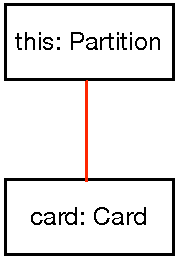
\includegraphics[width=0.2\textwidth]{goal_removeCard.pdf}
	\caption{Removing a card from its partition}
	\label{fig:goal_removeCard}
\end{figure}
\FloatBarrier

\vspace{0.5cm}

According to the signature of the method \texttt{removeCard}, we should return the card that has been deleted. Although this might strike you as slightly odd,
considering that we already passed in the card as an argument, it still makes sense as it allows for chaining method calls:
\syntax{ aPartition.removeCard(aCard).invert()}

Before we implement this change as a story diagram, let's remove the old injection content to avoid potential conflicts.

\begin{itemize}

\item[$\blacktriangleright$] Delete the \texttt{PartitionImpl.inject} file from your working set (\Cref{eclipse:delete_injection}).

\item[$\blacktriangleright$] Now select \texttt{LearningBoxLanguage} and click on the ``Build" button. 

\item[$\blacktriangleright$] You'll be able to see the changes in \texttt{PartitionImpl.java}. The \texttt{removeCard}
declaration should now be empty and look identical to the other unimplemented methods.

\end{itemize}

\newpage

\begin{figure}[htbp]
	\centering
    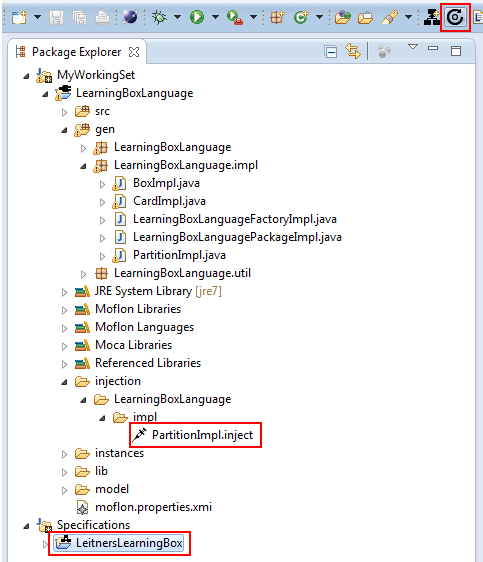
\includegraphics[width=0.5\textwidth]{eclipse_removeInjection}
	\caption{Remove injection content}
	\label{eclipse:delete_injection}
\end{figure}

\vspace{1cm}

That's it! We now have a fresh start for \texttt{removeCard}. Let's briefly discuss what we need to establish the transformation.

One of the goals of SDM is to allow you to focus less on \emph{how} a method will do something, but rather on \emph{what} the method will do.
Integrated as an atomic step in the overall control flow, a single graph transformation step (such as link deletion) can be embedded as a
\emph{story pattern}.

These patterns declare \emph{object variables}\define{Object \\ Variable}, place holders for actual objects in a model. During \emph{pattern matching}, objects
in the current model are assigned to the object variables in the pattern according to the indicated type and other conditions.\footnote{We shall learn what
further conditions may be specified in later SDMs.}

\clearpage

In \texttt{removeCard}, the SDM requires just two object variables: a \texttt{this} partition (named according to Java convention) referring to the
object whose method is invoked, and \texttt{card}, the parameter that will be removed.

Patterns also declare \emph{link variables}\define{Link \\ Variable} to match references in the model. Given that
we're concerned with removing a certain card from a specific partition, \texttt{removeCard} will therefore have a single link variable that connects these two
objects together.

In general, pattern matching is non-deterministic, i.e., variables in the pattern are bound to \emph{any} objects that happen to match. How can this
be influenced so that, as required for \texttt{removeCard}, the pattern matcher chooses the correct \texttt{card} (that which is passed in as a parameter)?

The \emph{binding state}\define{Binding~State} of an object variable determines how it is found. By default, every object variable is \emph{unbound}, or a 
\emph{free variable}\define{Free \\ Variable}. Values for these variables can be determined automatically by the pattern matcher. By declaring an
object variable that is to be \emph{bound}\define{Bound} however, it will have a fixed value determined from previous activity nodes. The appropriate binding is
implicitly determined via the \emph{name} of the bound object variable. As a rule, \texttt{this} variables, and any method parameters (i.e., \texttt{card}) are
always bound.

On a final note, every object or link variable can also set its \emph{binding operator} to \texttt{Check Only, Create, or Destroy}. For a rule $r: (L,
R)$, as discussed in \hyperlink{explanation}{Section 2}, this marks the variable as belonging to the set of elements to be retained ($L\cap R$), the set of
elements to be newly created ($R\setminus L$), or the set of elements to be deleted ($L\setminus R$).

If you're feeling overwhelmed by all the new terms and concepts, don't worry! We will define them again in the context of your chosen syntax with the
concrete example. For quick reference, we have also defined the most important terms at the end of this part in a \hyperlink{glossary}{glossary}. 


\newpage
\hypertarget{remCard vis}{}
\subsection{Implementing removeCard}
\visHeader

\begin{itemize}

\item[$\blacktriangleright$] Re-open the LearningBoxLanguage diagram in Enterprise Architect (EA) from Eclipse by double-clicking the \texttt{.eap}
file. Carefully do the following: (1) Click \emph{once} on \texttt{Partition} to select it, then (2) Click \emph{once} on the method
\texttt{removeCard} to highlight it (Fig.~\ref{fig:sdm_start}), and (3) \emph{Double-click} on the chosen method to indicate that you want to implement it.

\begin{figure}[htp]
\begin{center}
  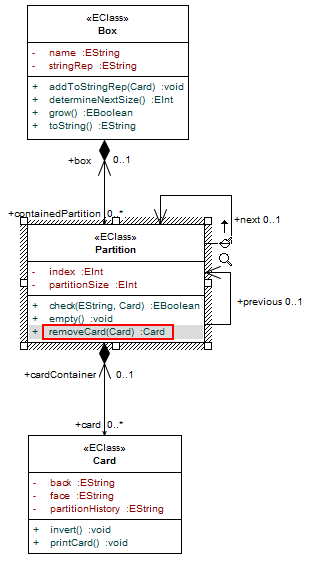
\includegraphics[width=0.6\textwidth]{ea_startSDM}
  \caption{Double-click a method to implement it}  
  \label{fig:sdm_start}
\end{center}
\end{figure}
 
\item[$\blacktriangleright$] If you did everything right, a new \emph{activity diagram} should be created and open in a new tab with a cute anchor in
the corner, and a \emph{start node} labelled with the signature of the method (Fig.~\ref{fig:sdm_skeleton}).  

\begin{figure}[htp]
\begin{center}
 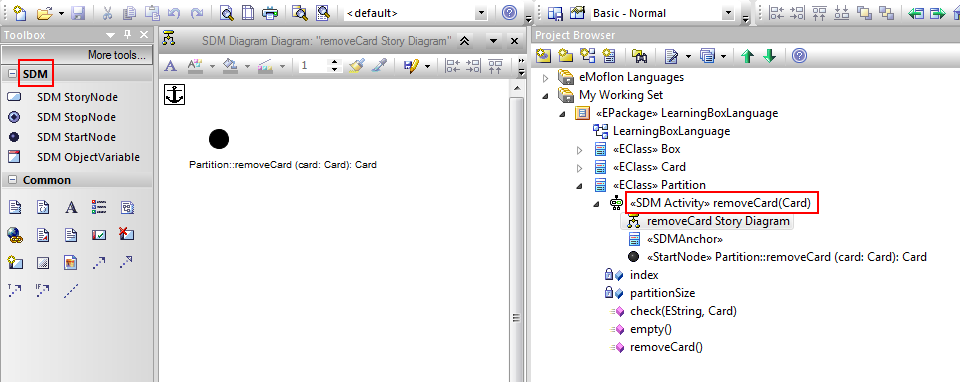
\includegraphics[width=1.0\textwidth]{ea_generatedSDM}
  \caption{Generated SDM diagram and start node}  
  \label{fig:sdm_skeleton}
\end{center}
\end{figure}

\vspace{0.5cm}

\item[$\blacktriangleright$] Let's quickly familiarise ourselves the EA workspace. First, inspect the project browser and notice that an \texttt{<<SDM
Activity>>} container has been created for the method \texttt{removeCard}. This container will eventually host every diagram related to this pattern. Please
note that, if you're at any time unhappy with an SDM,\footnote{As you might have already noticed, we use ``SDM'' interchangeably to mean our graph
transformation language \emph{or} a concrete transformation (a story model) used to implement a method and consisting of an activity diagram and a pattern in
each story node.} you can always delete the appropriate container in the project browser (such as this one), and start from scratch.

\vspace{0.5cm}

\item[$\blacktriangleright$] Next, note the new \texttt{SDM} toolbox that has been automatically opened for the diagram and placed to the left above
the common toolbox. This provides quick access to SDM items that you'll frequently use in your diagram.

\vspace{0.5cm}

\item[$\blacktriangleright$] Finally, in the top left corner of the diagram, you'll notice a small anchor. Double click on this icon to quickly jump back to the
metamodel. From there, double click the method again to jump back to the SDM. This is just a small trick to help you quickly shift between diagrams.

\vspace{0.5cm}

\item[$\blacktriangleright$] To begin, select the start node, and note the small black arrow that appears (Fig.~\ref{fig:sdm_quicklink}). 

\newpage

\begin{figure}[htp]
\begin{center}
  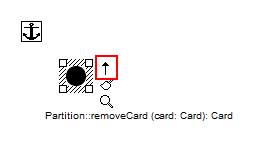
\includegraphics[width=0.5\textwidth]{ea_sdmStartNode}
  \caption{Quick link in SDM diagram to create new activity node}  
  \label{fig:sdm_quicklink}
\end{center}
\end{figure}

\item[$\blacktriangleright$] Similar to quick linking,\footnote{Learnt in Part II, Section 2.5} a second fundamental gesture in EA is \emph{Quick
Create}.
To quick-create an element, pull the arrow and click on an empty spot in the diagram. This is basically ``quick linking'' to a non-existent element.

\item[$\blacktriangleright$] EA notices that there is nothing to quick-link to, and pops a small context-sensitive dialogue to create an element that can be
connected to the indicated source element.

\item[$\blacktriangleright$] As illustrated in Fig.~\ref{fig:sdm_new_activity_node}, choose \texttt{Append StoryNode} to create an \emph{activity
node}. We refer to the whole activity diagram simply as the \emph{activity}, which always starts with a start node, terminates with a \emph{stop node}, and
consists of activity nodes connected via \emph{activity edges}.

\begin{figure}[htp]
\begin{center}
  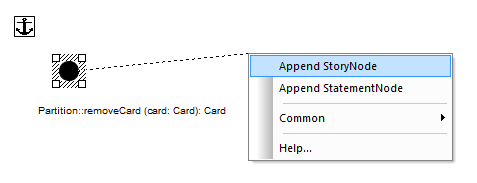
\includegraphics[width=0.8\textwidth]{ea_sdmQuickLinkStoryNode}
  \caption{Create new activity node}  
  \label{fig:sdm_new_activity_node}
\end{center}
\end{figure}

\item[$\blacktriangleright$] If you quick-created correctly, you should now have a start node, an activity node called \texttt{ActivityNode 1}, and an edge
connecting the two items. Complete the activity by quick creating a stop node as depicted in Fig.~\ref{fig:sdm_stop_node}.

\begin{figure}[htp]
\begin{center}
  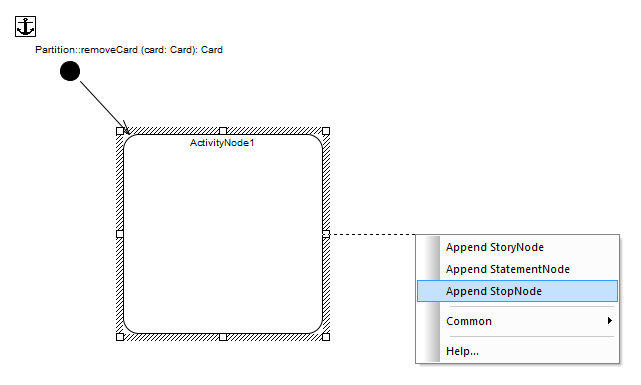
\includegraphics[width=\textwidth]{ea_sdmAppendStopNode}
  \caption{Complete activity with a stop node}  
  \label{fig:sdm_stop_node}
\end{center}
\end{figure}

\vspace{0.5cm}

\item[$\blacktriangleright$] If everything is correct, you should now have a complete activity that models the \emph{control flow} of the method. 
The semantics of our activity is pretty straightforward -- the control begins in the start node, and flows along edges and their connected activity nodes until
it reaches a stop node, where it finally terminates. 

\vspace{0.5cm}

\item[$\blacktriangleright$] While a \emph{stop node} is rather self explanatory, you may be wondering about the differences between the other two item options,
a\define{Story Node}\emph{story node}and a \emph{statement node}.\define{Statement Node}Since not all activity nodes can contain story patterns (i.e., start
and stop nodes), those that \emph{can} are called story nodes. Statement nodes are simply used to guarantee a certain action. They happen between story nodes.
We'll encounter these in a later SDM, but for now, lets finish our first story node.

\vspace{0.5cm}

\item[$\blacktriangleright$] To craft the story pattern, double click \texttt{ActivityNode 1} to prompt the dialogue depicted in
Fig.~\ref{fig:story_pattern}. Enter \texttt{removeCardFromPartition} as the name of the story node, and select \texttt{Create this Object}.  Click
\texttt{OK} - the activity node now has a single \emph{object variable}, \texttt{this} (Fig.~\ref{fig:tool_box}).

\begin{figure}[htpb]
\begin{center} 
  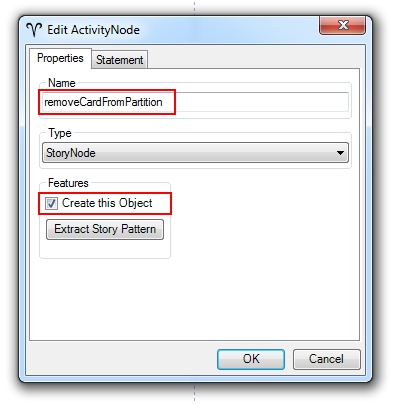
\includegraphics[width=0.6\textwidth]{ea_sdmEditActivityNode}
  \caption{Start modelling story pattern in activity node}  
  \label{fig:story_pattern}
\end{center}
\end{figure}

\begin{figure}[htp]
\begin{center}
  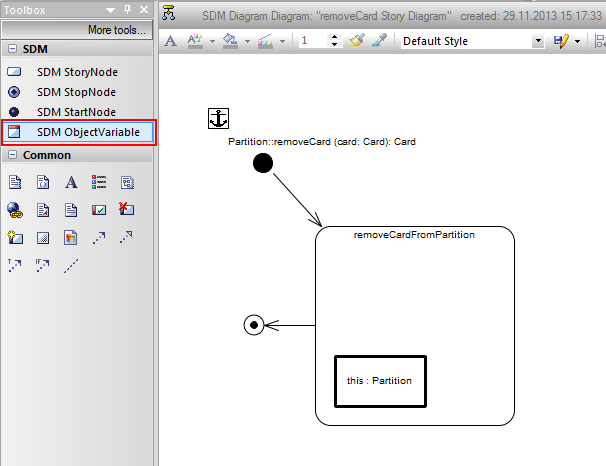
\includegraphics[width=0.8\textwidth]{ea_sdmNewObjVar}
  \caption{Add a new object variable from the toolbox}  
  \label{fig:tool_box}
\end{center}
\end{figure}

\newpage

\item[$\blacktriangleright$] To create an object variable that can be assigned to other objects, either choose \texttt{SDM ObjectVariable} from the toolbox or
press \texttt{ctrl}, then click inside the activity node (Fig.~\ref{fig:tool_box}). A properties window will be raised for the new object
(Fig.~\ref{fig:object_variable_properties}).

\vspace{0.5cm}

\begin{figure}[htp]
\begin{center}
  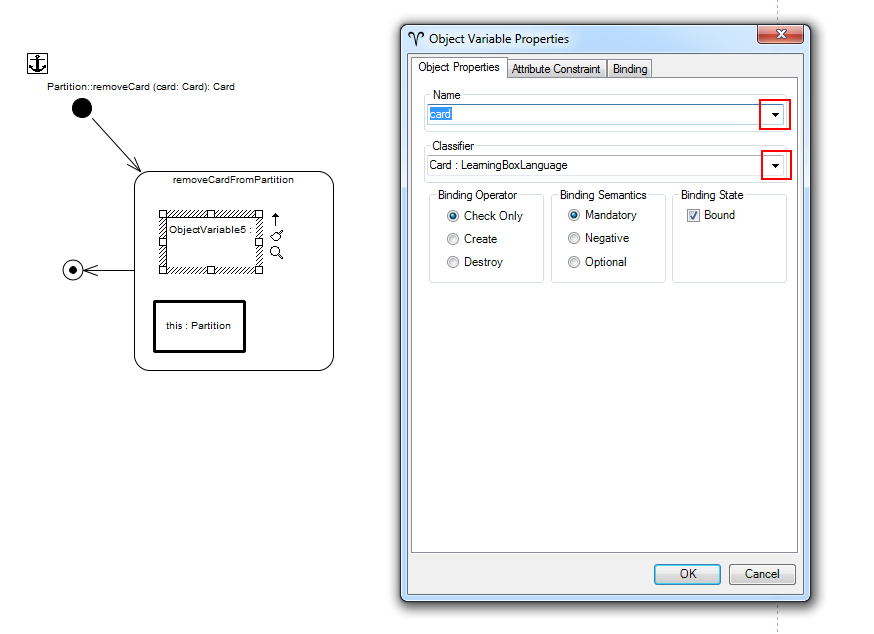
\includegraphics[width=\textwidth]{ea_sdmPropertiesObjVar}
  \caption{Specify properties of the added object variable}  
  \label{fig:object_variable_properties}
\end{center}
\end{figure}


\item[$\blacktriangleright$] Using the drop-down menus, choose \texttt{card} as the name of the object variable and set \texttt{Card} as its type.
Since \texttt{card} is a parameter of the method, it is offered as a possible name which can be directly chosen to prevent annoying typing mistakes.

\vspace{0.5cm}

\item[$\blacktriangleright$] In this dialogue, note that the \texttt{Bound} option must be set. We have now seen two cases in this activity for bound object
variables: an assignment to \texttt{this}, and an assignment to a method parameter. \texttt{Unbounded} object are represented by a thin-bordered box. Setting
\texttt{card} to bound means that it will implicitly assign itself to the passed parameter valued.

\item[$\blacktriangleright$] To create a \emph{link variable} between the current partition and the card to be removed, choose the object variable \texttt{this}
and quick-link it to \texttt{card} (Fig.~\ref{fig:link_variable}).

\begin{figure}[htpb]
\begin{center}
  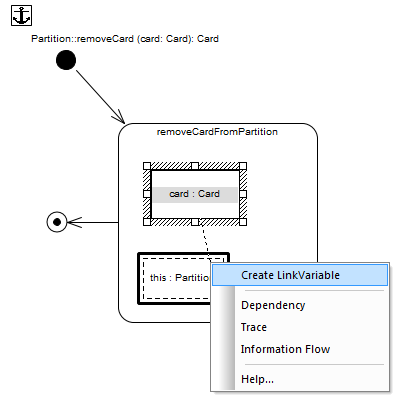
\includegraphics[width=0.6\textwidth]{ea_sdmCreateLinkVar}
  \caption{Create a link variable}   
  \label{fig:link_variable}
\end{center}
\end{figure}

\item[$\blacktriangleright$] According to the metamodel, there is only one possible link between a partition and card. Select this and set the
\emph{Binding Operator} to \texttt{Destroy} (Fig.~\ref{fig:link_variable_properties}). The reference names will automatically appear in the diagram.

\vspace{0.5cm}

% Had to force (h!) image to appear here; no other images were co-operating
\begin{figure}[h!]
\begin{center} 
 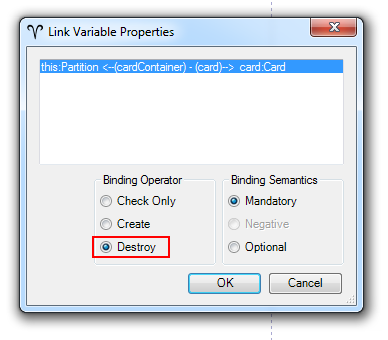
\includegraphics[width=0.6\textwidth]{ea_sdmBindLink}
  \caption{Specify properties for created link variable}  
  \label{fig:link_variable_properties}
\end{center}
\end{figure}

\vspace{0.5cm}

\item[$\blacktriangleright$] Remember how we said that this method should return the same card that was passed in? As luck would have it, a return value for any
SDM can be specified in the stop node. As depicted in Fig.~\ref{fig:stop_node_return_value}, double-click the stop node to prompt the \texttt{Edit StopNode} dialogue. 

\begin{figure}[htbp]
\begin{center}
  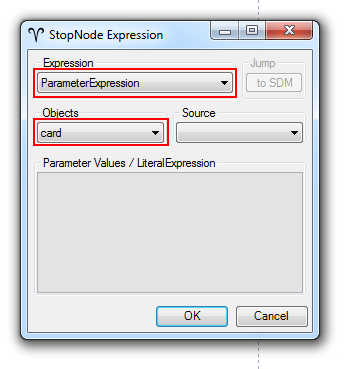
\includegraphics[width=0.5\textwidth]{ea_sdmStopNodeExpr}
  \caption{Adding a return value to the stop node}  
  \label{fig:stop_node_return_value}
\end{center}
\end{figure}

\item[$\blacktriangleright$] In the \texttt{Expression} field, choose \texttt{ParameterExpression}\define{ParameterExpression}as the expression. Given that
\texttt{card} is the sole parameter, it will be automatically selected. In EA, a \emph{ParameterExpression} is a mechanism that exclusively accesses any
paramter value.

\vspace{0.5cm}

We're nearly done! As you can see, by using several different dialouges, eMoflon employs a simple context-sensitive expression language for specifying required
values. We have intentionally avoided creating a full-blown sub-language, and limit expressions to a few simple types.\footnote{We also do not support nesting
expressions} The philosophy here is to keep things simple and concentrate on what SDMs are good for -- expressing structural changes. Our approach is to
provide a clear and type-safe interface to a general purpose language (Java) and support a simple \emph{fallback} as soon as things get too low-level and
difficult to express as a pattern.

The alternative approach to eMoflon would be to support arbitrary expressions, for example, in a script language like JavaScript or in an appropriate
DSL\footnote{A DSL is a Domain Specific Language: a language designed for a specific task which is usually simpler than a general purpose language like Java and
more suitable for the exact task.} designed for this purpose. In the following SDM implementations, we'll learn the other expression types eMoflon supports,
and how to use them. 

\item[$\blacktriangleright$] Returning to the activity, if you've done everything right, your first SDM completed with eMoflon should resemble
Fig.~\ref{fig:sdm_complete_control_flow}. The return value is indicated below the stop node.


\begin{figure}[htbp]
\begin{center}
  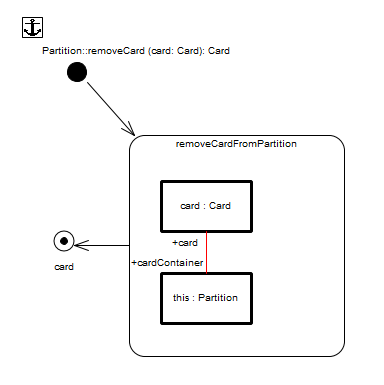
\includegraphics[width=0.7\textwidth]{ea_sdmRemoveComplete}
  \caption{Complete SDM for \texttt{Partition::removeCard}}  
  \label{fig:sdm_complete_control_flow}
\end{center}
\end{figure}

\item[$\blacktriangleright$]  Don't forget to save your files, validate and export your pattern to the Eclipse workspace,\footnote{Go to to
``\texttt{Extensions}" and select \texttt{Add-In Windows} to activate eMoflon's console. If you're unsure how to validate, export, or use this window, review
Part II, section 3} then build your metamodel's code from the package explorer.

\item[$\blacktriangleright$] If you're unable to export or generate code successfully, compare your SDM carefully with Fig.~\ref{fig:sdm_complete_control_flow}
and make sure you haven't forgotten anything.

\item[$\blacktriangleright$] If successful, navigate to ``Learning\-Box\-Language/\-gen/\-Learning\-Box\-Language/\-impl/\-Partition\-Impl.java" to the
\texttt{\-remove\-Card} declaration. Inspect the generated implementation for your method. Notice all the null checks that are automatically created - only a
very conscientious (and probably slightly paranoid) programmer would program so defensively!

Let's take a step back and briefly review what we have specified:  if \texttt{p.remove\-Card(c)} is invoked for a partition \texttt{p}, with a card, \texttt{c},
as its argument, the specified pattern will \emph{match} only if that card is contained in the partition. After determining matches for all variables, the
link between the partition and the card is deleted, effectively ``removing'' the card from the partition. If the card is \emph{not} contained in the partition,
the pattern won't match, and nothing will happen. In both cases, the card that's passed in is returned.

\item[$\blacktriangleright$] If you'd like to see how this SDM is implemented in the textual syntax, check out Fig.~\ref{fig:deleteReference} in the next
section.

\item[$\blacktriangleright$] Now we admit, this section had a lot of reading and theory, but it does get better. Soon, you'll be an eMoflon master, and we'll
hardly need to give you any instructions at all! In the following sections, we shall explore further features of SDM that allow for really expressive and
powerful patterns.

\fancyfoot[R]{ $\triangleright$ \hyperlink{sec:checkCard}{Next} }

\end{itemize}



\newpage
\genHeader
\hypertarget{remCard end}{}
\subsubsection{Concluding removeCard}

Fantastic work! You have now implemented a simple method via patterns. As you can see, SDMs are effective for implementing structural changes in a high-level,
intuitive manner.

Let's take a step back and briefly review what we have specified:  if \texttt{p.remove\-Card(c)} is invoked for a partition \texttt{p}, with a card \texttt{c}
as its argument, the specified pattern will \emph{match} only if that card is contained in the partition. After determining matches for all variables, the
link between the partition and the card is deleted, effectively ``removing'' the card from the partition. If the card is \emph{not} contained in the partition,
the pattern won't match, and nothing will happen. In both cases, the card that's passed in is returned.

\begin{itemize}

\item[$\blacktriangleright$] If your code generation was successful, navigate to
``Learning\-Box\-Language/\-gen/\-Learning\-Box\-Language/\-impl/\-Partition\-Impl.java" to the \texttt{\-remove\-Card} declaration (approximately line 352).
Inspect the generated implementation for your method (Fig.~\ref{fig:remCardImpl}). Notice the null checks that is automatically created - only a very
conscientious (and probably slightly paranoid) programmer would program so defensively!

\vspace{0.5cm}

\begin{figure}[htp]
\begin{center}
  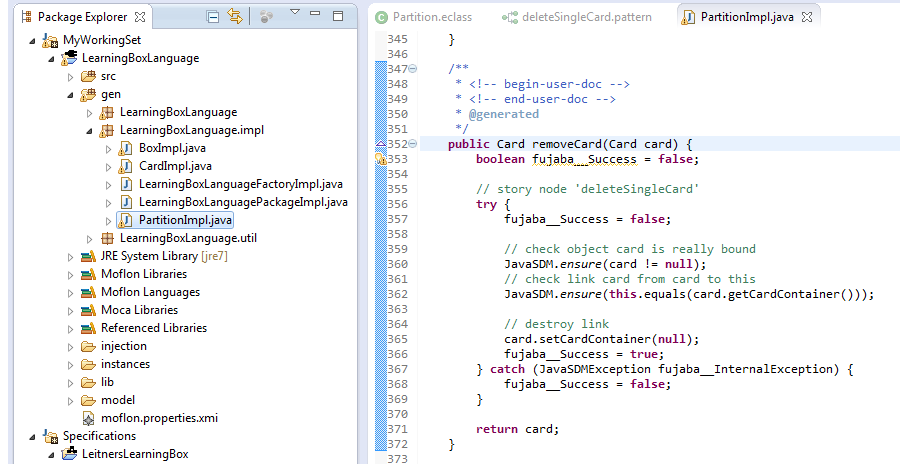
\includegraphics[width=\textwidth]{eclipse_remCardImpl}
  \caption{Generated implementation code}
  \label{fig:remCardImpl}
\end{center}
\end{figure}

\newpage

Near the end of Part II (after using injections), you were able to test this method's implementation using our \texttt{LeitnersBoxGui}. Let's run it again to
make sure \emph{this} version of \texttt{removeCard} works!

\item[$\blacktriangleright$] Load and run the GUI as an application,\footnote{Refer to Part II, Section 6 for details on our GUI} then go to any partition and
select \texttt{Remove Card} (Fig.~\ref{fig:GUIRemCard}).
It should immediately refresh, and you'll no longer be able to see the card in either the GUI or in the \texttt{Box.xmi} tree in the ``instances'' folder.
Pretty cool, eh?

\vspace{1cm}

\begin{figure}[htp]
\begin{center}
  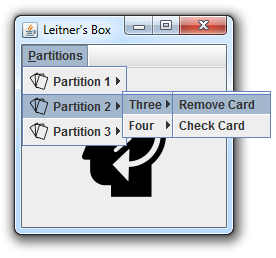
\includegraphics[width=0.5\textwidth]{eclipse_GUIRemove}
  \caption{Testing \texttt{removeCard}}
  \label{fig:GUIRemCard}
\end{center}
\end{figure}

\end{itemize}



\newpage
\hypertarget{sec:checkCard}{}
\section{Checking a card}
\genHeader

The next method we shall model is probably the most important for our learning box. This method will be invoked when a user decides to test themselves on a card
in the learning box. They'll be able to see the \texttt{back} attribute of a card from the box, make a guess as to what's on the \texttt{face}, then 
check their answer (\Cref{fig:goal_check}). Following our rules established in \Cref{fig:membox_depiction}, if their guess was correct the card will be
\emph{promoted} to the next partition. If wrong, the card will be \emph{penalized} and returned to the first.

\begin{figure}[htbp]
 	\centering
   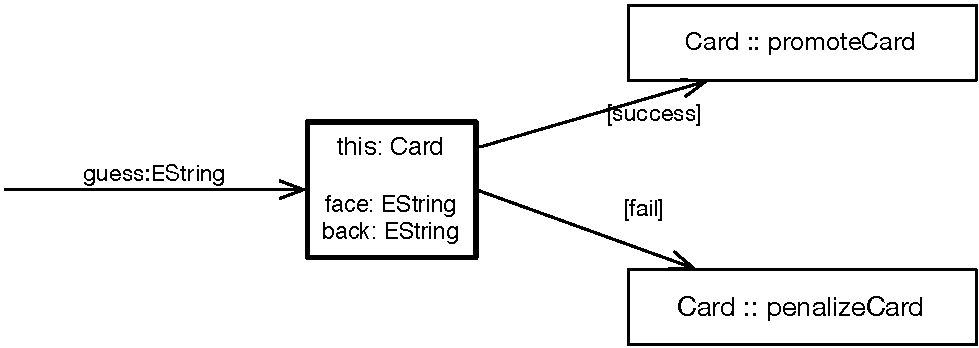
\includegraphics[width=0.7\textwidth]{goal_checkCard.pdf}
 	\caption{Checking a card with a guess}
 	\label{fig:goal_check}
\end{figure}
\FloatBarrier

As you can see, checking \texttt{guess} is a simple assertion on string values. The actual movements of the card however, must be implemented as separate
patterns. \Cref{fig:patterns_check} briefly shows the intended create and destroy transformations.

\begin{figure}[htbp]
 	\centering
   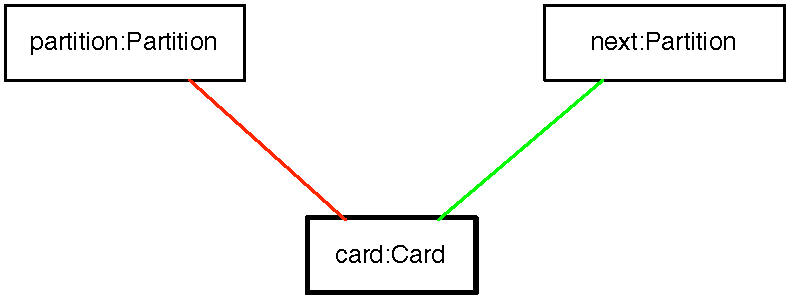
\includegraphics[width=0.5\textwidth]{checkCard_promote.pdf}
   \\ \vspace{1cm}
    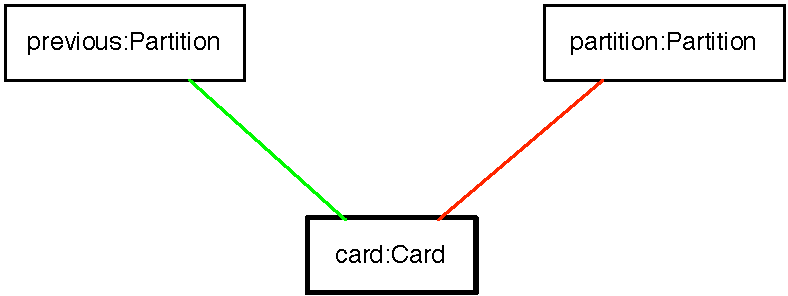
\includegraphics[width=0.5\textwidth]{checkCard_penalize.pdf}
 	\caption{Promote (above) and penalize (below) card patterns}
 	\label{fig:patterns_check}
\end{figure}
\FloatBarrier

Overall, this means the control flow must utilize an \emph{if/else} construct. The \texttt{guess} conditional also needs to be an \emph{attribute
constraint}\define{Attribute Constraint}, a non-structural condition that must be satisfied in order for a story pattern to match. 

\newpage
\subsection{Implementing check}
\visHeader
\hypertarget{checkCard vis}{}

\begin{itemize}

\vspace{1cm}

\item[$\blacktriangleright$] Since you're nearly a SDM wizard already, try using concepts we have already learnt to create the control flow for
\texttt{Partition::check} as depicted in Fig.~\ref{fig:sdm_check_start}.

\vspace{1cm}

\begin{figure}[htbp]
\begin{center}
  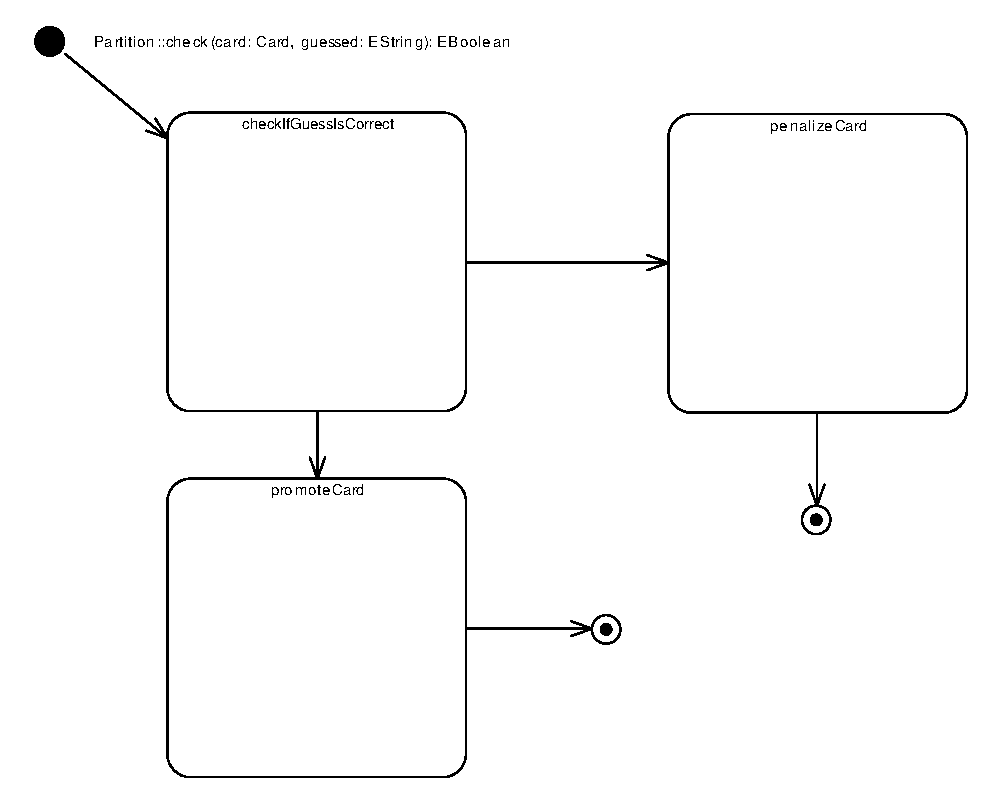
\includegraphics[width=1\textwidth]{ea_activityCheck.pdf}
  \caption{Activity diagram for \texttt{Partition::check}}
  \label{fig:sdm_check_start}
\end{center}
\end{figure}

\vspace{1cm}

\item[$\blacktriangleright$] In \texttt{checkIfGuessIsCorrect}, create an object variable that is bound to the parameter argument, \texttt{card} 
(Fig.~\ref{fig:sdm_check_addCard}). This will represent the card the user picked from the learning box. Remember, the binding for this variable is implicitly
defined when its name is the same as the argument's name.

\begin{figure}[htbp]
\begin{center}
  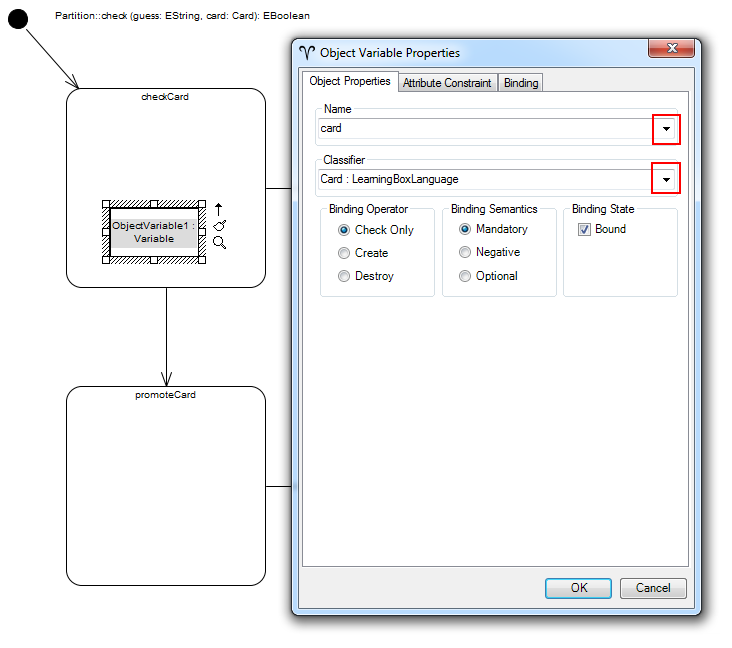
\includegraphics[width=\textwidth]{ea_addObjVarCard}
  \caption{Creating the card variable}
  \label{fig:sdm_check_addCard}
\end{center}
\end{figure}

\clearpage

\item[$\blacktriangleright$] Now that the pattern has the correct card to check, it needs to compare the user's guess against the unseen \texttt{face} value on
the opposite side. To do this, we need to specify an \emph{attribute constraint}. Open the \texttt{attribute constraint} tab as depicted in
Fig.~\ref{fig:sdmcheck_att_constraint}, select the correct object attribute (\texttt{face}) and comparison operator.

\begin{figure}[htbp]
\begin{center}
  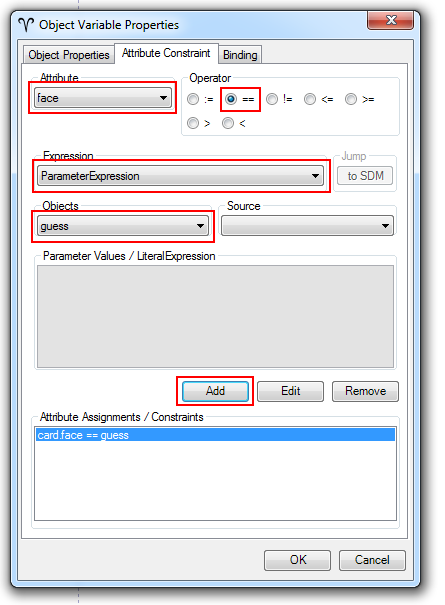
\includegraphics[width=0.6\textwidth]{ea_addAttConst}
  \caption{Creating an attribute constraint}
  \label{fig:sdmcheck_att_constraint}
\end{center}
\end{figure}

\item[$\blacktriangleright$] Similar to how the return value was specified in the previous SDM, set the \texttt{ParameterExpression} to refer to \texttt{guess}.
Press \texttt{Add} and admire your first attribute constraint.

\vspace{1cm}

Before building the other two activity nodes, let's quickly return to the control flow. Currently, the pattern will branch off into two separate patterns after
completing the initial check, then terminate the method based on whichever activity finishes first\ldots and that's not what we want at all! We need to add
\emph{edge guards} to change this into an \emph{if/else} construct based on the results of the comparison.

\newpage

\item[$\blacktriangleright$] To add a guard to the edge leading from \texttt{check\-If\-Guess\-Is\-Correct} to \texttt{penalize\-Card}, double click the edge
and set the \emph{Guard Type} to \texttt{Failure} (Fig.~\ref{fig:sdm_check_guard}).

\vspace{0.5cm}

\begin{figure}[htbp]
\begin{center}
  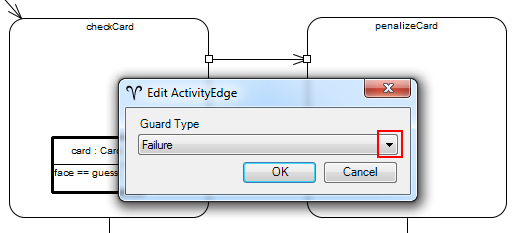
\includegraphics[width=0.75\textwidth]{ea_addTransitionGuard}
  \caption{Add a transition with a guard}
  \label{fig:sdm_check_guard}
\end{center}
\end{figure}

\vspace{0.5cm}

\item[$\blacktriangleright$] Repeat the process for the \texttt{Success} edge leading to \texttt{promoteCard}.

\vspace{0.75cm}

Another feature of eMolfon (with EA) provides a means of coping with large patterns.\footnote{You thought I was going to say `coping
with our coffee addiction', weren't you?} It might be nice to visualise \emph{small} story patterns directly in their nodes, but for large patterns or complex
control flow, such diagrams would get extremely cumbersome and unwieldy very quickly! This is indeed a popular argument against visual languages and it might
have already crossed your mind (``This is cute, but it'll \emph{never} scale!''). With the right tools and concepts however, even huge diagrams can be
mastered. We support \emph{extracting} story patterns into their own diagrams, and unless the pattern is really concise with 2 or 3 object variables, recommend
this course of action.

\vspace{0.5cm}

\item[$\blacktriangleright$] To try this, double-click the \texttt{promoteCard} story node and choose \texttt{Extract Story Pattern}
(Fig.~\ref{fig:sdm_check_extract_storypattern}). Note the new diagram that is immediately opened and created in the project browser
(Fig.~\ref{fig:sdm_new_sub_diagram}).

\begin{figure}[htbp]
\begin{center}
  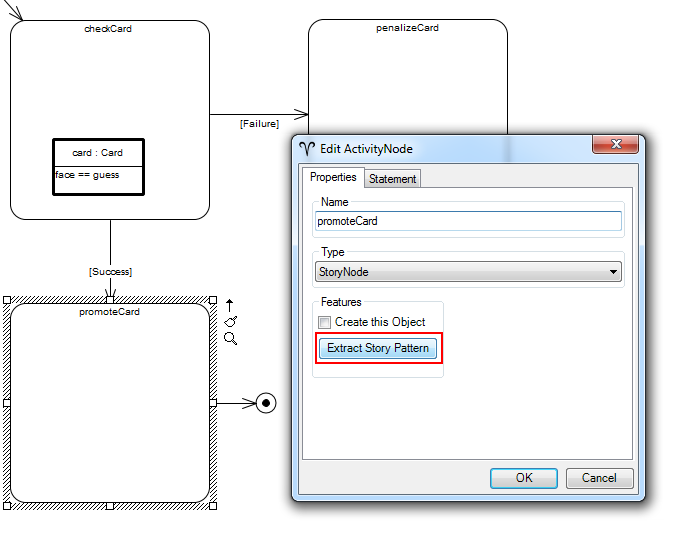
\includegraphics[width=0.8\textwidth]{ea_extractStoryPattern}
  \caption{Extract a story pattern for more space and a better overview}
  \label{fig:sdm_check_extract_storypattern}
\end{center}
\end{figure}

\begin{figure}[htbp]
\begin{center}
  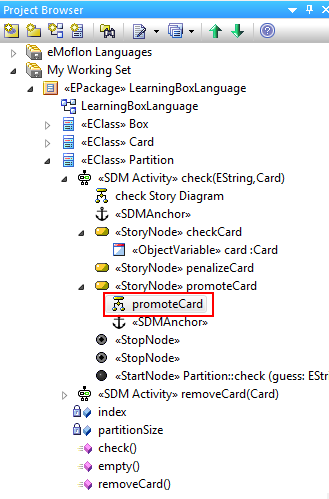
\includegraphics[width=0.45\textwidth]{sdm_promoteCardProjBrowser}
  \caption{A new sub diagram is created automatically}
  \label{fig:sdm_new_sub_diagram}
\end{center}
\end{figure}

\newpage

Another EA gesture you should start to take advantage of is a good ol' \emph{Drag and Drop} action from the project browser\footnote{Remember he other two
gestures we have learnt: ``Quick Link'' and ``Quick Create''.} into a diagram. We can use this move as an alternative to creating new objects (with known types) from the SDM
toolbox.

\vspace{0.5cm}

\item[$\blacktriangleright$] To create a new \texttt{Card} object variable, simply drag and drop the class from the project browser into the new (extracted)
pattern diagram (Fig.~\ref{fig:sdm_check_bound_card}).

\begin{figure}[htbp]
\begin{center}
  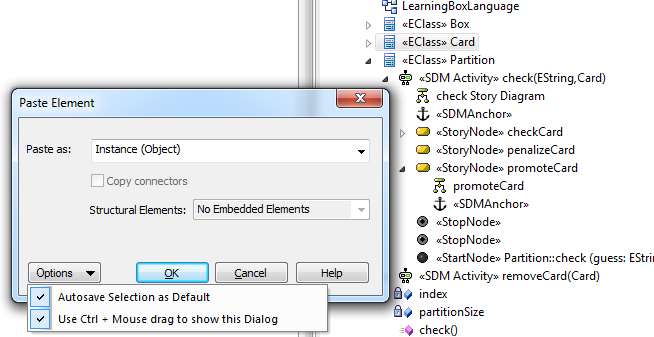
\includegraphics[width=0.8\textwidth]{ea_dragDropDialogue}
  \caption{Add a new object variable per drag and drop}
  \label{fig:sdm_check_bound_card}
\end{center}
\end{figure}

\item[$\blacktriangleright$] A dialogue will appear asking what kind of variable should be created. You can create (1) a simple link (which would
refer to and be represented by \texttt{Card}'s class), (2) create an instance of \texttt{Card} as an object, or (3) create a subclass. Paste \texttt{Card} as an
instance and check \texttt{Autosave Selection as Default} under ``Options" so option (2) will be used next time by default. You should also check \texttt{Use
Ctrl + Mouse drag to show this Dialog}, so this dialogue doesn't appear every time. Don't worry - if you ever need options (1) and (3), you  just need to hold
\texttt{Ctrl} when dragging to invoke the dialogue then change the settings.

\vspace{0.5cm}

\item[$\blacktriangleright$] After creating the object, the same object properties dialogue will open.  Set the \texttt{Name} to `card' and its \texttt{Binding
State} to ``Bound'' (Fig.~\ref{fig:sdm_new_card_properties}).

\newpage

\begin{figure}[htbp]
\begin{center}
  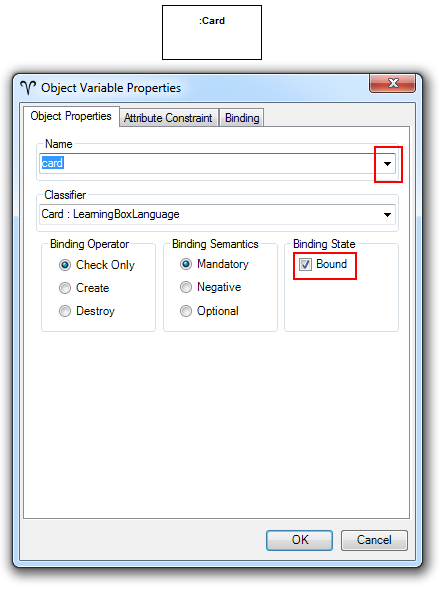
\includegraphics[width=0.5\textwidth]{ea_addBoundObj}
  \caption{Object variable properties of the new card}
  \label{fig:sdm_new_card_properties}
\end{center}
\end{figure}

The main advantage of drag and drop is that the \texttt{Object Variable Pro\-per\-ties} dialogue should have the type of the object pre-configured. Choosing
the type in the project browser and dragging it in is (for most people) a more natural gesture than choosing the type from a long drop-down menu (as we had to
when using the SDM toolbar). This can be a great time saver for large metamodels\footnote{Drag and drop is also possible in embedded story patterns
(still visualised in their story nodes).  You must ensure however, that the object variable is \emph{completely} contained inside the story node and does not
stick out over any edge}.

\vspace{0.5cm}

\item[$\blacktriangleright$] Currently, we have the single \texttt{card} that we want to promote through the box. Drag and drop two further object variables for
the current partition, \texttt{this}, and the \texttt{nextPartition} as depicted in Fig.~\ref{fig:sdm_check_complete_sp}.

\begin{figure}[htbp]
\begin{center}
  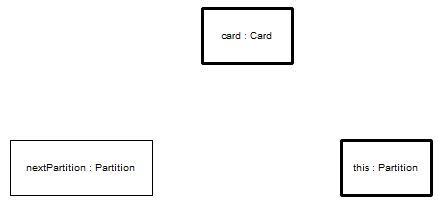
\includegraphics[width=0.8\textwidth]{ea_promoteCardVariables}
  \caption{All object variables for story pattern \texttt{promoteCard}}
  \label{fig:sdm_check_complete_sp}
\end{center}
\end{figure}

\vspace{0.5cm}

An important point to note here is that \texttt{this} and \texttt{card} are visually differentiated from \texttt{nextPartition} by
their bold border lines. This is how we differentiate \emph{bound} from \emph{unbound} (\emph{free}) variables. We already know that matches for bound
variables are completely determined by the current context. On the other hand, matches for unbound variables, have to be determined by the pattern matcher. Such
matches are ``found'' by navigating and searching the current model for possible matches that satisfy all specified constraints (e.g. type of the variable,
links connecting it to other variables and attribute constraints). In our case, the next partition will have to be determined by navigating from \texttt{this}
via the \texttt{next} link in the metamodel.

\vspace{0.5cm}

\item[$\blacktriangleright$] Quick link from \texttt{this} to \texttt{nextPartition} (or vice-versa) to create a \texttt{next} link variable, as shown in
Fig.~\ref{fig:sdm_check_link_variable}. As you can see, there are several more property options. The goal is to have the current partition to proceed or point
to the \texttt{nextPartition} via the \texttt{next} reference, so select the second option. This will cause the reference to be defined in \texttt{this}.
Alternatively, you could define the reference in \texttt{nextPartition} by setting the link proceed from the next partition into the \texttt{previous}
partition, \texttt{this}.

\begin{figure}[htbp]
\begin{center}
  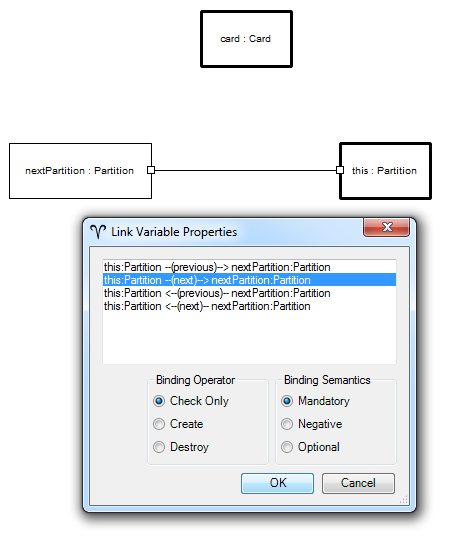
\includegraphics[width=0.85\textwidth]{ea_promoteLinkProperties}
  \caption{Connecting \texttt{this} and \texttt{nextPartition}}
  \label{fig:sdm_check_link_variable}
\end{center}
\end{figure}

\vspace{0.5cm}

\item[$\blacktriangleright$] Continue creating links between \texttt{card} and each partition. Remember - you want to \emph{destroy} the reference to
\texttt{this}, and \emph{create} a new connection to \texttt{nextPartition}. If everything is set up correctly, \texttt{promoteCard} should now closely resemble
Fig.~\ref{fig:sdm_check_complete_activity_node}.

\begin{figure}[htbp]
\begin{center}
  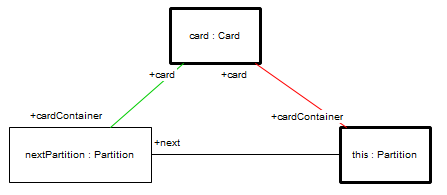
\includegraphics[width=0.8\textwidth]{ea_promoteCardCompleted}
  \caption{Complete story pattern for \texttt{promoteCard}}
  \label{fig:sdm_check_complete_activity_node}
\end{center}
\end{figure}

\clearpage

\item[$\blacktriangleright$] Double click the anchor in the top left corner and repeat the process for \texttt{penalizeCard}: First extract the story pattern,
then create the necessary variables and links as depicted in Fig.~\ref{fig:sdm_check_complete_penalize}. As you can see, this pattern is nearly identical to
\texttt{promoteCard}, except it moves the card to a \texttt{previousPartition}.

\vspace{0.5cm}

\begin{figure}[htbp]
\begin{center}
  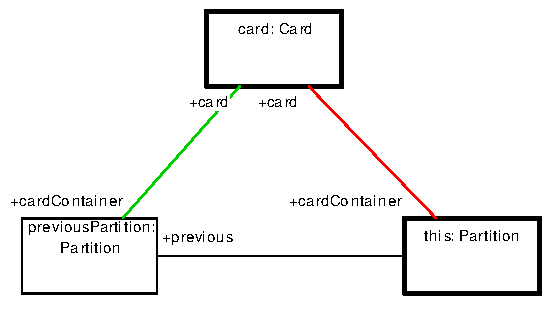
\includegraphics[width=0.8\textwidth]{ea_completeActivityPenalize.pdf}
  \caption{Story pattern for activity node \texttt{penalizeCard}}
  \label{fig:sdm_check_complete_penalize}
\end{center}
\end{figure}


\vspace{0.5cm}

To complete the \texttt{check} SDM, we need to signal (as a return value) the result of the check - was the card promoted or penalised? To do this, we need to
edit the stop nodes so they return a\define{LiteralExpression}\emph{LiteralExpression}. This expression type can be used to specify arbitrary text, but
should really only used for true literals like 42, ``foo'' or \texttt{true}. It can be (mis)used for formulating any (Java) expression that will simply be
transferred ``literally'' into the generated code, but this is obviously sort of dirty\footnote{It defeats, for example, any attempt to guarantee type safety}
and should be avoided when possible.

\item[$\blacktriangleright$] To implement a literal, double click the stop node stemming from  \texttt{promoteCard}, and change the expression type from
\texttt{void} to \texttt{LiteralEx\-pression} (Fig.~\ref{fig:sdm_check_literal_exp}). Change the value in the window below to \texttt{true}. Press \texttt{OK},
then finish the SDM by returning \texttt{false} after \texttt{penaliseCard} in the same manner. Your diagram should now resemble
Fig.~\ref{fig:sdm_check_finish}.

\begin{figure}[htbp]
\begin{center}
  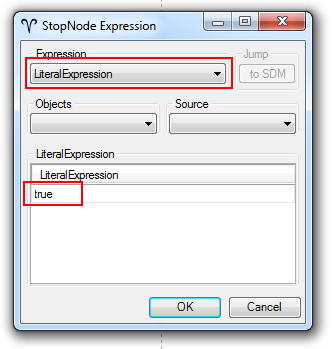
\includegraphics[width=0.5\textwidth]{ea_stopNodeLiteral}
  \caption{Add a return value with a literal expression}
  \label{fig:sdm_check_literal_exp}
\end{center}
\end{figure}

\begin{figure}[htbp]
\begin{center}
  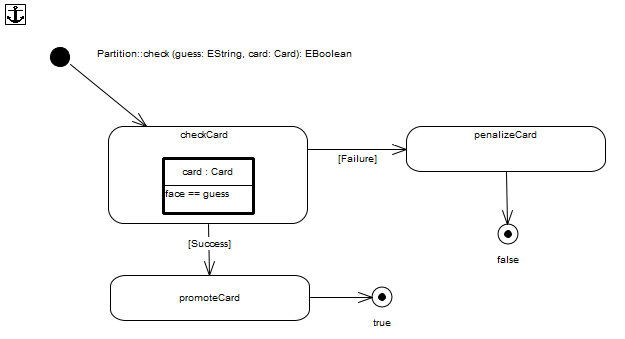
\includegraphics[width=\textwidth]{ea_sdmCheckComplete}
  \caption{Complete SDM for \texttt{Partition::check}}
  \label{fig:sdm_check_finish}
\end{center}
\end{figure}

\clearpage

\item[$\blacktriangleright$] Great job - the SDM is now complete! Validate and export your project, then inspect the implementation code for \texttt{check}. We
strongly recommend that you even write a simple JUnit test (take a look at our simple test case from Part I for inspiration) to take your brand new SDM for a
test-spin.

\item[$\blacktriangleright$] To see how this is implemented in the textual syntax, see Figs. \ref{fig:completedPatterns} and \ref{fig:finalMethod} in the
following section.

\fancyfoot[R]{ $\triangleright$ \hyperlink{sec:emptyPartition}{Next}}

\end{itemize}



\newpage
\hypertarget{sec:extendGui}{}
\section{Extending the Leitner's Box GUI}
\genHeader

\vspace{0.5cm}

In addition to \texttt{removeCard}, the GUI is able to access and operate the \texttt{check} method using your SDM implementation! To avoid build errors
however, it was originally commented out so you'll need to release it. First, double check and make sure your metamodel is built, and that you have correctly
imported the GUI.\footnote{Review how to download and run the GUI in Part II, section 6}

\begin{itemize}

\item[$\blacktriangleright$] Go to ``Other Projects/LeitnersBox/Src'' and open \texttt{Leitners\-Box\-Cont\-roller\-.java} in the package.

\vspace{0.5cm}

\item[$\blacktriangleright$] On the far right side of the editor, you should be able to see two blue rectangles in the space beside the scrollbar. Click on the
second to skip ahead to the \texttt{check} command (Fig.~\ref{fig:remComment}).

\vspace{0.5cm}

\begin{figure}[htp]
\begin{center}
  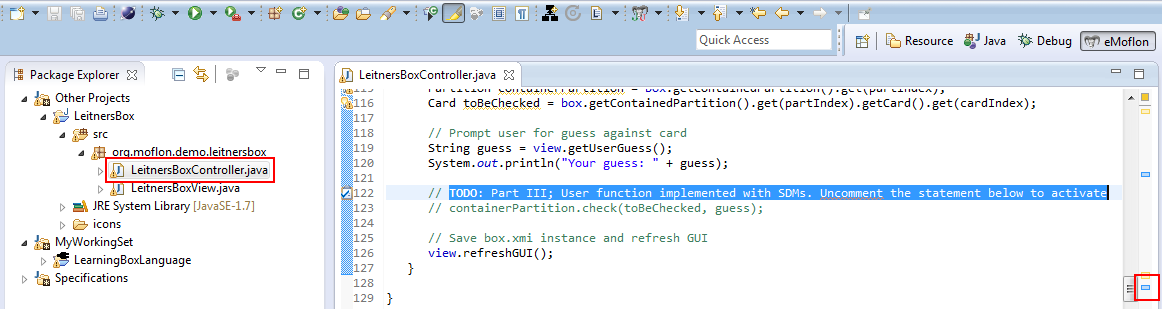
\includegraphics[width=\textwidth]{eclipse_GUICommentLine}
  \caption{Remove the comment operator on line 123}
  \label{fig:remComment}
\end{center}
\end{figure}

\vspace{0.5cm}

\item[$\blacktriangleright$] Remove the commented line below the \texttt{TODO} statement, save the file, then take your GUI for a spin! Experiment with
making right and wrong guesses, and watch how your cards move through the box. Try editing your instance file by making more partitions, cards and some
new \texttt{FastCard}s to see how they behave.

\end{itemize}


\newpage
\hypertarget{sec:emptyPartition}{}
\section{Emptying a partition of all cards}
\genHeader

This next SDM should \emph{empty} a partition by removing every card contained within it. Since we can assume that there is more than one card in the
partition,\footnote{If there was only one, we would just invoke \texttt{removeCard}} we obviously need some construct for repeatedly deleting each card in the
partition (Fig.~\ref{fig:goal_empty}). 

\begin{figure}[htbp]
	\centering
  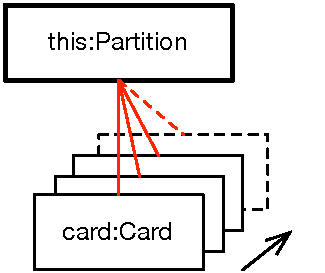
\includegraphics[width=0.3\textwidth]{goal_partitionEmpty.pdf}
	\caption{Emptying a partition of every card}
	\label{fig:goal_empty}
\end{figure}
\FloatBarrier

In SDM, this\define{For Each}construct is accomplished via a \emph{for each} story node. It performs the specified actions for \emph{every} match of its
pattern (i.e., every \texttt{Card} that matches the pattern will be deleted). This however, gives us two interesting points to discuss.
Firstly, how would the pattern be interpreted if the story node were a normal, simple control flow node, not a \emph{for each} node?

The pattern would specify that \emph{a} card should be matched and deleted from the current partition - that's it. The \emph{exact} card is not specified,
meaning that the actual choice of the card is \emph{non-deterministic} or random, and it is only done once. This randomness is a common property of both graph
transformations and pattern matching, and it's something that takes time getting used to.  In general, there are no guarantees concerning the choice and
order of valid matches. The \emph{for each} construct however, ensures that \emph{all} cards will be matched and deleted.

Our second point is determining if we actually need to destroy the link between \texttt{this} and \texttt{card}. Would the pattern be interpreted differently if we
destroyed \texttt{card} and left the link?

The answer is no, the pattern would yield the same result, regardless if the link is explicitly destroyed!\define{Dangling Edges}This is due to the
transformation engine eMoflon uses.\footnote{CodeGen2, a part of the Fujaba toolsuite \url{http://www.fujaba.de/}} It ensures that there are never any
\emph{dangling edges} in a model. Since deleting just the \texttt{card} would result in a dangling edge attached to \texttt{this}, that link is deleted as well. Explicitly
destroying the links as well is therefore a matter of taste, but \ldots why not be as explicit as possible?

\jumpDual{emptyPartition vis}{emptyPartition tex}

\newpage
\subsection{Implementing empty}
\visHeader
\hypertarget{emptyPartition vis}{}

\begin{itemize}
\vspace{0.5cm}

\item[$\blacktriangleright$] To create a \emph{for each} story node in EA, create the initial diagram and start node for the method \texttt{Partition::empty},
then \emph{quick create} an activity node choosing \texttt{ForEach} as its type (Fig.~\ref{fig:sdm_foreach}). A \emph{for each} story node is visualised as a
double node to indicate potential repetition.

\vspace{1cm}

\begin{figure}[htbp]
\begin{center}
  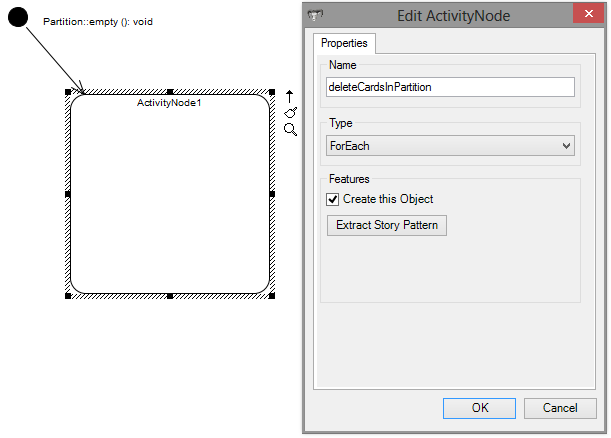
\includegraphics[width=0.9\textwidth]{ea_forEach}
  \caption{A for each loop in SDM.}  
  \label{fig:sdm_foreach}
\end{center}
\end{figure}

\vspace{1cm}

\item[$\blacktriangleright$] Next, complete the story pattern as indicated in Fig.~\ref{fig:sdm_end}. Please note that the \texttt{card} that is deleted in each match
is unbound, and both the \texttt{card} and link to \texttt{this} are set to \texttt{destroy}. Even more important, notice that the guard that terminates the for
each story node has an \texttt{[end]} guard. Indeed, a \emph{for each} story node \emph{must} have an end activity edge which is taken when all matches for the
story pattern have been handled.

\pagebreak

\begin{figure}[htbp]
\begin{center}
  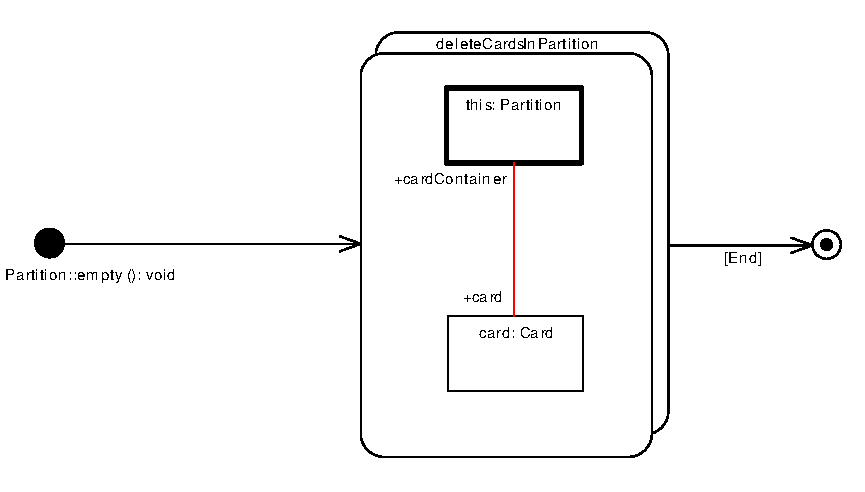
\includegraphics[width=0.9\textwidth]{ea_completeActivityEmptyCards.pdf}
  \caption{Complete story pattern with \texttt{[end]} guard.}  
  \label{fig:sdm_end}
\end{center}
\end{figure}

\fancyfoot[R]{ $\triangleright$ \hyperlink{sec:invertCard}{Next SDM} } \item[$\blacktriangleright$] Done! That's all we needed to do to specify a repeating
action. Pretty simple, eh? Inspect Figs. \ref{fig:emptyControlFlow} and \ref{fig:emptyPattern} to see how this is implemented textually.

\end{itemize}



\newpage
\hypertarget{emptyPartition tex}{}
\subsection{Implementing empty}
\texHeader

\begin{itemize}
 
\item[$\blacktriangleright$] To initialize your new control flow, you can once again take advantage of eMoflon's auto completion. Inside the
\texttt{empty} declaration, press  \texttt{Ctrl + Space} and select
\texttt{forEach} from the menu (Fig.~\ref{eclipse:typeCompletion}).

\vspace{1cm}

\begin{figure}[htpb]
\begin{center}
  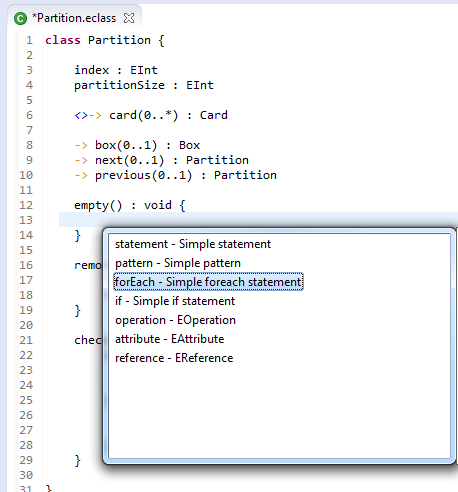
\includegraphics[width=0.7\textwidth]{eclipse_emptyTypeCompletion}
  \caption{eMoflon's auto completion}
  \label{eclipse:typeCompletion}
\end{center}
\end{figure}

\vspace{1cm}

\item[$\blacktriangleright$] Create a single pattern, \texttt{deleteCardsInPartition}. Remove the suggested second pattern as you only need to complete the
deletion -- no extra steps are required in this simple case!

\item[$\blacktriangleright$] Your activity should now resemble Fig.~\ref{eclipse:emptyControlFlow}.

\clearpage

\begin{figure}[htpb]
\begin{center}
  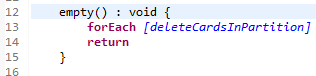
\includegraphics[width=0.5\textwidth]{eclipse_emptyControlFlow}
  \caption{Control flow for \texttt{partition.empty()}}
  \label{eclipse:emptyControlFlow}
\end{center}
\end{figure}

\item[$\blacktriangleright$] While similar to \texttt{removeCard} (Fig.~\ref{eclipse:deleteReference}), this new pattern will go one step further by requesting
a full destruction of \texttt{card}, instead of just deleting the link between the object variables. This means that in addition to destroying the link between
the partition and \texttt{card}, we need to destroy the object variable \texttt{card} as well.

\item[$\blacktriangleright$] Create a \texttt{@this} object variable, and delete its link to \texttt{card} via \syntax{-- -> card:card} Then create another
object variable \texttt{card}, deleting it by prefixing its name with the same \texttt{`--'} operator.

\vspace{0.5cm}

\item[$\blacktriangleright$] Your pattern should now resemble Fig.~\ref{eclipse:emptyPattern}.

\vspace{0.5cm}

\begin{figure}[htpb]
\begin{center}
  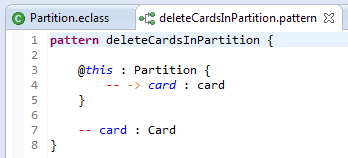
\includegraphics[width=0.6\textwidth]{eclipse_emptyPattern}
  \caption{Destroying both \texttt{card} and the link variable}
  \label{eclipse:emptyPattern}
\end{center}
\end{figure}

\vspace{0.5cm}

\item[$\blacktriangleright$] That's it! Look at you go\ldots you're just speeding through these SDMs now! To see how \texttt{empty} is specified in the visual
syntax, review Fig.~\ref{ea:sdm_end} from the previous section.

\vspace{0.5cm}

\item[$\blacktriangleright$] Although the Learning Box GUI does not have an explicit action that invokes this SDM, feel free to extend it and see your SDM in
action!

\end{itemize}


 
\newpage
\hypertarget{sec:invertCard}{}
\section{Inverting a card}
\genHeader

This next SDM \emph{inverts} a card by swapping its back and face values (Fig.~\ref{fig:goal_invert}). This therefore ``turns a card around'' in the learning
box. This action makes sense if a user wants to try learning, for example, the definition of a word in the other (target) language. Instead of guessing the
definition of every word when presented with the term, perhaps they would like to guess the term when presented with the definition. This method doesn't need to
accept any parameters -- it'll use a bound \texttt{this} variable.

\vspace{0.5cm}

\begin{figure}[htbp]
	\centering
    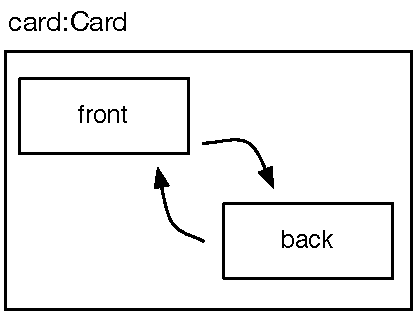
\includegraphics[width=0.4\textwidth]{goal_invert.pdf}
 	\caption{Inverting the attributes of a \texttt{Card}}
 	\label{fig:goal_invert}
\end{figure}
\FloatBarrier

Something new that we'll use in this SDM are \emph{assignments}\define{Assignments}to set the attributes of \texttt{temp} to the \texttt{card}, then again to
set \texttt{card} to the `new' swapped values. An assignment is simply an attribute constraint\footnote{Which we first encountered in \texttt{check}} set via a
`\texttt{:=}' operator. Though it may be slightly confusing to refer to an assignment as a constraint, if you think about it, \emph{everything} can be
considered as a constraint that must be fulfilled through different strategies.

With \texttt{invert}, a successful match is achieved not by searching as you would with a comparison (\texttt{==, >, <, \ldots}), but by \emph{performing} the
above assignment. If the assignment cannot be completed, the match is invalid. Similarly, non-context elements (set to create or destroy) can be viewed as
structural constraints that are fulfilled when the corresponding element is created or destroyed.  A constraint is therefore a unifying concept similar to
``everything is an object'' from OO, and ``everything is a model'' from metamodelling.  If you're interested in why \emph{unification} is considered cool check
out \cite{BEZ05}.

\jumpDual{invertCard vis}{invertCard tex}

\newpage
\hypertarget{invertCard vis}{}
\subsection{Implementing invert}
\visHeader

\begin{itemize}

\vspace{0.5cm}

\item[$\blacktriangleright$] If you've completed all the work so far, you've got to be \emph{really} good at SDMs now. Model the simple story diagram
depicted in Fig.~\ref{ea:sdm_invertEmpty}.

\vspace{0.5cm}

\begin{figure}[htbp]
\begin{center}
  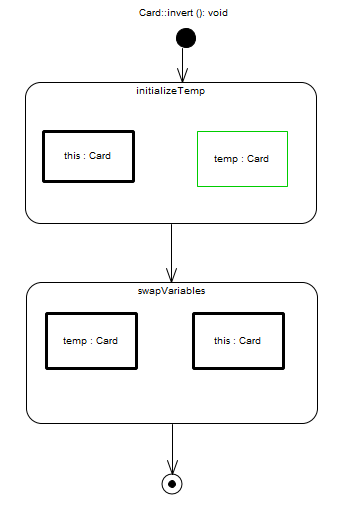
\includegraphics[width=0.6\textwidth]{ea_invertEmpty}
  \caption{Imperative control layer for inverting a card}  
  \label{ea:sdm_invertEmpty}
\end{center}
\end{figure}

\item[$\blacktriangleright$] Note that the binding operator on the first \texttt{temp} object variable is set to \texttt{create} (thus the green
border). This means that we actually \emph{create} a new object, and do not pattern match to an existing one in our model.

\item[$\blacktriangleright$] This activity will need four assignment constraints - two in \texttt{in\-it\-ia\-lize\-Temp} (to store the ``opposite'' values),
and two in \texttt{swapVariables} (to switch the values). Create your first assignment constraint by going to the created \texttt{temp} card and using the
`\texttt{:=}' operator to set the \texttt{temp.back} value to \texttt{this.face} (Fig.~\ref{ea:sdm_invertAssignment}).

\begin{figure}[htbp]
\begin{center}
  \includegraphics[width=0.7\textwidth]{ea_invertAttConstAssign}
  \caption{Store the \texttt{back} and \texttt{face} values of the card in \texttt{temp}}  
  \label{ea:sdm_invertAssignment}
\end{center}
\end{figure}

\clearpage

\vspace*{0.5cm}

\item[$\blacktriangleright$] Complete the SDM with the remaining constraints according to Fig.~\ref{ea:sdm_invertComplete} below.

\vspace{0.5cm}

\begin{figure}[htbp]
\begin{center}
  \includegraphics[width=0.7\textwidth]{ea_invertComplete}
  \caption{Swap back and face of the card}  
  \label{ea:sdm_invertComplete}
\end{center}
\end{figure}

\vspace{0.5cm}

\item[$\blacktriangleright$] Believe or not, that's it! Check out how this method is implemented in the textual syntax by reviewing
Fig.~\ref{eclipse:invertPatterns} in the next section. You don't \emph{have} to export and build to Eclipse, but it's always nice to confirm your work is error
free.

\jumpSingle{invert close} 

\end{itemize}


\newpage
\subsection{Textual; Turning Cards}
\texHeader
\hypertarget{invertCard tex}{}

Fill

\newpage
\subsubsection{Inversion review}
\genHeader
\hypertarget{invert close}{}

Before we start the next SDM, let's quickly review one point. Have you considered why the \texttt{temp} object variable is bound in the second pattern for
\texttt{invert}, (\texttt{swap variables}), but not where it's first defined in \texttt{initialize temp}?\footnote{See \Cref{ea:sdm_invertComplete}} This is a new case for bound variables that we haven't treated yet!

Until now, we have seen object variables that can be bound to (1) an argument of the method (set when the method is invoked), or (2) the
current object (\texttt{this}) whose method is invoked. In both cases, the object to be matched is completely determined by the context of the method before
the pattern matcher starts. This means that it does not need to be determined or found by the pattern matcher.

Setting \texttt{temp} as bound in \texttt{Swap variables} is a third case in which an object variable is bound to a value determined in a \emph{previous}
activity node without using a special expression type. In this SDM, this means \texttt{temp} will be bound to the value determined for a variable
of the same name in the previous node, \texttt{Initialize temp}. This binding feature enables you to refer to previous matches for object variables in the
preceding control flow.

On a separate note, you're just over halfway through completing this part of the eMoflon handbook, so give your brain a small break. Take a walk, pour
yourself another coffee, and check out one of my favourite jokes:
\syntax{How do you wake up Lady Gaga?}

\vspace{0.5cm}

\syntax{Poke her face!}




\newpage
\section{Growing the box}
\genHeader

Ok, back to business. In this SDM, we shall explicitly specify how our learning box is to be built up. We create a specific pattern that will append new
partition elements to the end of a \texttt{Box} that follow our established movement rules (\Cref{fig:membox_depiction}). This means the new partition will
become the \texttt{next} reference of the current last partition, and its \texttt{previous} reference must be connected to the first partition in the box
(\Cref{fig:goal_grow}).

\begin{figure}[htbp]
 	\centering
  	\includegraphics[width=0.7\textwidth]{growBoxNACGoal.pdf}
	\caption{Growing a box by inserting a new partition}
	\label{fig:goal_grow}
\end{figure}
\FloatBarrier

SDMs provide a declarative means of identifying specific partitions via \emph{Negative Application Conditions}, simply referred to as
\mbox{NAC}s.\footnote{Pronounced $\backslash 'nak \backslash$}\define{NAC} \mbox{NAC}s express structures that are forbidden to exist before applying a
transformation rule. In this SDM, the \mbox{NAC} will be an object variable that must not be assigned a value during pattern matching. In the theory of
algebraic graph transformations \cite{EEPT06}, \mbox{NACs} can be arbitrarily complex graphs that are much more general and powerful than what we currently
support in our implementation,\footnote{To be precise, in CodeGen2 from Fujaba} namely only single negative elements (object or link variables).

As depicted in \Cref{fig:goal_grow}, to create an appropriate \mbox{NAC} that constrains possible matches, we'll need to check to see if the currently
matched pattern can be extended to include the negative elements. Suppose the current potential last partition has a \texttt{nextPartition}. This means it
is \emph{not} the absolute last partition, and so the match becomes invalid. We only want to insert a new partition when the \texttt{nextPartition}
of the current potential last partition is null. Similarly, if the current potential first partition has a \texttt{previousPartition}, the match is invalid. The
complete match is therefore made unique through NACs and thus becomes \emph{deterministic} by construction. In other words, if you \emph{grow} the box with this method, there
will always be exactly one first and one last partition of the box.

Of course, to complete this method we still need to determine the size of the new partition. Since the size must be calculated depending on the
rest of the partitions currently in the box (partitions usually get bigger) we'll need to call a helper method, \texttt{determineNextSize} via a
\emph{MethodCallExpression}\define{MethodCallExpression}. As the name suggests, it is designed to access any method defined in \emph{any} class in the current
project.

Due to the algorithmic and non-structural nature of \texttt{determineNextSize}, it will be easier to implement this method via a Java \emph{injection}, rather
than an SDM. We've already declared this method in our metamodel, so its signature will be available for editing in \texttt{BoxImpl.java}.

\begin{itemize}

\item[$\blacktriangleright$] Open ``gen/LearningBoxLanguage.impl/BoxImpl.java.'' Scroll to the method declaration, and replace the contents with the code in
\Cref{code:determineNextSize_impl}. Remember not to remove the first comment, which is necessary to indicate that the code is handwritten and needs to be
extracted automatically as an injection. Please do not copy and paste the following code -- the copying process from your pdf viewer to the Eclipse IDE
will likely add invisible characters to the code that eMoflon is unable to handle.

\begin{figure}[htbp]
        \centering
        \begin{lstlisting}[language=Java, keywordstyle={\bfseries\color{purple}}, backgroundcolor=\color{white}]
    public int determineNextSize() {
    	// [user code injected with eMoflon]
        return getContainedPartition().size()*10;
    }
        \end{lstlisting}
        \caption{Implementation of \texttt{removeCard}}
        \label{code:determineNextSize_impl}
\end{figure}


\item[$\blacktriangleright$] Save the file, then right-click on it, either in the package explorer or in the editor window, and choose ``eMoflon/
Create/Update Injection for class'' from the context menu. 

\item[$\blacktriangleright$] Confirm the update in the new \texttt{BoxImpl.inject} file's partial class. \texttt{determineNextSize} is now ready to be used by
your metamodel!

\end{itemize}

\newpage
\subsection{Implementing grow}
\visHeader
\hypertarget{growBox vis}{}

\begin{itemize}
 
\item[$\blacktriangleright$] Start by creating the simple story pattern depicted in Fig.~\ref{fig:sdm_grow_1}. This matches the box
(\texttt{this}), with \emph{any} two partitions in the box\footnote{Remember, this is for the \emph{pattern matcher}}.

\begin{figure}[htbp]
\begin{center}
  \includegraphics[width=\textwidth]{ea_elementsGrowBox.pdf}
  \caption{Context elements for SDM}  
  \label{fig:sdm_grow_1}
\end{center}
\end{figure}

\item[$\blacktriangleright$] To create the appropriate \mbox{NAC} (to constrain the possible matches for \texttt{lastPartitionInBox}),  create the new object
variable \texttt{nextPartition}, of type \texttt{Partition}, and set \note{Binding Semantics} its \emph{Binding Semantics} to \texttt{negative}
(Fig.~\ref{fig:sdm_grow_2}). The object variable should be visualised as being cancelled or struck out. % why?
 
\begin{figure}[htbp]
\begin{center}
  \includegraphics[width=0.9\textwidth]{ea_negElement}
  \caption{Adding a negative element}  
  \label{fig:sdm_grow_2}
\end{center}
\end{figure}
 
\item[$\blacktriangleright$] Now, quick link \texttt{nextPartition} to \texttt{lastPartitionInBox}, but be sure choose the link type carefully! The
\texttt{nextPartition} should play the role of \texttt{next} with respect to \texttt{lastPartitionInBox}.

\item[$\blacktriangleright$] Complete the story pattern so that it closely resembles Fig.~\ref{fig:sdm_grow_3}. 

\begin{figure}[htbp]
\begin{center}
  \includegraphics[width=\textwidth]{ea_NACFirstLast.pdf} 
  \caption{Determining the first and last partition with NACs}  
  \label{fig:sdm_grow_3}
\end{center}
\end{figure}
 
\item[$\blacktriangleright$] Notice how the created partition \texttt{newPartition} is `hung' into the box. It becomes the next partition of the current
\emph{last} partition, and has its previous partition set to the first partition in the box (as depicted with the arrows in Fig.~\ref{fig:membox_depiction}).
  
\item[$\blacktriangleright$] To complete this SDM, build the assignment to set the size of the new partition. Go ahead and invoke the corresponding dialogue to
activate the \texttt{:=} operator.

Given that the new size must be calculated using a helper function via a \emph{MethodCallExpression}.\define{MethodCallExpression}A MethodCallExpression is
used to invoke a method defined in any class in the current EA project. Enter the values in Fig.~\ref{fig:sdm_grow_4}, choosing the argument \texttt{this} as
the target, and \texttt{determineNextSize} as the method to be invoked. 

Since \texttt{determineNextSize} doesn't require any parameters, you can ignore the \texttt{Parameters} field this time, but for future reference, parameters
can be specified by choosing the appropriate parameter declaration between guillemets (e.g. \texttt{<Box box>}) found in the drop-down menu and typing in the
value (this is basically a literal expression). Don't forget to press the \texttt{Save} button for every parameter, then \texttt{Add} + \texttt{OK} to confirm
and close the dialogue.
 
 %UPDATE not under 'target' but 'objects'
\begin{figure}[htbp]
\begin{center}
  \includegraphics[width=0.5\textwidth]{ea_methodCall.png}
  \caption{Invoking a method via a \texttt{MethodCallExpression} {\bf UPDATE}}  
  \label{fig:sdm_grow_4} 
\end{center}
\end{figure}

\item[$\blacktriangleright$]  If you've done everything right, your SDM should now closely resemble Fig.~\ref{fig:sdm_grow_5}. 

% As usual, try to export, generate code, inspect the
% method implementation and write a JUnit test.  This time around you also have to
% implement the helper method \texttt{determineNextSize} directly in the
% generated code
% (\texttt{gen/\-LearningBoxLanguage/\-facade/\-impl/\-LearningBoxUtilImpl}).
% Don't forget to add \texttt{@generated NOT} to the Java doc comment of the
% method so the code generator preserves your code in future runs.
% When testing (which you will \emph{of course} do right?), note that you can only grow a ``minimal'' box that has at least a first and last partition, i.e., a box with 
%no partitions at all cannot be grown using our specified SDM. 

\begin{figure}[htbp]
\begin{center}
  \includegraphics[width=0.9\textwidth]{ea_completeActivityGrowBox.pdf}
  \caption{Complete SDM for \texttt{Box::grow}}  
  \label{fig:sdm_grow_5}
\end{center}
\end{figure}

\item[$\blacktriangleright$]  That's it - your \texttt{grow} SDM is complete! This was probably the most challenging SDM to build, so give yourself a solid 
pat on the back. If you found it easy then \ldots gee whiz, I don't think i'm doing my job correctly. To see how this is done in the texual syntax, review
Fig.~\ref{fig:patternComplete}.\footnote{We do recommend reading the instructions for this one, however, since NACs can be tricky.}

\end{itemize}



\newpage
\hypertarget{sec:conBran}{}
\section{Conditional Branching}

\footnotetext{\bf See page xvii of the old handbook for original. This is all new.}

When working with SDMs, you'll often find yourself needing to decide which statement(s) to execute based on the return value of an arbitrary (black box)
operation. In our example so far, we have implemented these constructs via SDM \emph{pattern matching}. 

With eMoflon however, there is an alternate way to
construct these black boxes. In fact, this feature is yet another way of integrating handwritten java code with your SDM! The only ``rule'' of this feature is that your
method must return \texttt{EBoolean}, \texttt{Success}, or \texttt{Failure}, respectively corresponding to \texttt{true} and \texttt{false}. Any other values
will set \texttt{Failure} to \texttt{null}. It follows that void methods cannot be used for branching - an exception will be thrown during execution.

Introduce example here; source has basic idea for \texttt{Check} modification.

% Suppose we wanted to modify \texttt{check} so that, instead of doing an exact comparison of \texttt{card.face} against \texttt{guess}, LeitnersBox prompts the
% user with the face of the card, then asks the user if their answers match. The user can then respond \texttt{yes} or \texttt{no}.\footnote{While you may
% initially consider this as an easy way to cheat (``They'll just say `yes' to everything!''), this is reflective of a true flashcard system. There can be several
% ways to provide the right answer, but \texttt{card.face} can only store one.}
% 
% Go to your \texttt{Partition.eclass} in the metamodel and create a new method, \texttt{isAnswer(card:Card, guess:EString):EBoolean}. Build and generate your
% files, then go to \texttt{PartitionImpl.java} (Fig.~\ref{fig:genIsAnsw}) and fill in the declaration with the code below (Fig.~\ref{}).\footnote{We are assuming you
% are unfamilar with JFrame, and have enabled this text to be easily copy/pasted into your Java file to avoid mistakes}
% 
% \begin{figure}[htp]
% \begin{center}
%   \includegraphics[width=\textwidth]{eclipse_generatedIsAnswer}
%   \caption{Generated code location for \texttt{isAnswer}}
%   \label{fig:genIsAnsw}
% \end{center}
% \end{figure}

% Second CODE figure with stuff that works (with gui)


\fancyfoot[R]{ $\triangleright$ \hyperlink{conBran vis}{Next [visual]\hspace{0.2cm} } \\ $\triangleright$ \hyperlink{conBran tex}{Next [textual]} } 

\clearpage
\hypertarget{conBran vis}{}
\subsection{Branching with statement nodes}
\visHeader

\begin{itemize}
  
\item[$\blacktriangleright$] Edit the \texttt{Box} class in your metamodel by invoking the \texttt{Operations} dialogue and create a new method called
\texttt{initalizeBox}. Recalling the sole condition of conditional branching, set its return type to \texttt{EBoolean}. Save the method, then re-open the
\texttt{grow} SDM.

\vspace{0.5cm}

\item[$\blacktriangleright$] Add a new \texttt{StatementNode} from \texttt{addNewPartitionBox} and name it \texttt{initialize}. The edge guard should
automatically set itself to \texttt{failure}.

\vspace{0.5cm}

\item[$\blacktriangleright$] In the \texttt{Statement} tab, invoke a \texttt{MethodCallExpression} to your new method.

\vspace{0.5cm}

\item[$\blacktriangleright$] Finally, attach two \texttt{StopNode}s -- \texttt{true} and \texttt{false} -- along with their appropriate edge guards. These mean
that the if method call succeeds, the box could be initialized, so it will return a literal \texttt{true}. If it failed however, \texttt{box} was already in an
invalid state (by, i.e., having only one card) and returns \texttt{false}. Overall, the new additions to \texttt{box.grow()} should resemble
Fig.~\ref{fig:newGrowControl}.

\vspace{0.5cm}

\begin{figure}[htp]
\begin{center}
  \includegraphics[width=\textwidth]{ea_growAdditions}
  \caption{Extending \texttt{grow} with a \emph{MethodCallExpression}}
  \label{fig:newGrowControl}
\end{center}
\end{figure}

\clearpage

\item[$\blacktriangleright$] Switch back to your open \texttt{Box.grow} SDM in EA. You'll notice that if you double-click on \texttt{initialize}, the
\texttt{Extract Story Pattern} option is invalid. This makes sense -- you don't define a pattern in a statement node. Instead, return to the main diagram and
create a new SDM for \texttt{initializeBox}.

\item[$\blacktriangleright$] In its diagram, create an \texttt{activity node} named \texttt{buildPartitions}. Within it, have a bound \texttt{Box} linked to a
\texttt{onePartition} NAC, and two other `green' (create) object variables, \texttt{firstPartition} and \texttt{lastPartition}. Be sure to also connect two
true/false \texttt{StopNode}s. The pattern should now resemble Fig.~\ref{fig:buildPartitions}. The NAC here can only fulfilled if the box has no partitions,
i.e., is in a pristine state and able to be initialized. In other words, If \texttt{grow} is used for an empty box, it initializes the box for the first time
and grows it after that, ensuring that the box is always in a valid state.

\vspace{0.5cm}
 
\begin{figure}[htp]
\begin{center}
  \includegraphics[width=\textwidth]{eclipse_buildPartitions}
  \caption{Compelted NAC to check for \emph{one} partition}
  \label{fig:buildPartitions}
\end{center}
\end{figure}
 
\item[$\blacktriangleright$] You're finished! Save, validate, and build your metamodel, then check out how this is done in the textual syntax in
Fig.~\ref{fig:updateGrow} and Fig.~\ref{fig:pattBuildParts}.

\jumpSingle{initialize notes}

\end{itemize}


\newpage
\hypertarget{conBran tex}{}
\subsection{Branching with statement nodes}
\texHeader

\begin{itemize}

\item[$\blacktriangleright$] Before doing anything else, let's declare the method that will insert two new partitions into \texttt{box} when the original
pattern match fails. Open \texttt{Box.eclass} and add the following signature anywhere in the file: 
\syntax{initializeBox() : EBoolean}

\vspace{0.5cm}

\item[$\blacktriangleright$] Now modify \texttt{Box.grow()} by adding a nested \emph{if/Else} construct, with \texttt{[addNewPartitionBox]} as the
first conditional, and execute a \emph{statement node} if it fails. \texttt{grow} should now resemble Fig.~\ref{fig:updateGrow}.

\vspace{0.5cm}

\begin{figure}[htp]
\begin{center}
  \includegraphics[width=0.5\textwidth]{eclipse_updateGrow}
  \caption{Extending \texttt{Box} with a \emph{statement node}}
  \label{fig:updateGrow}
\end{center}
\end{figure}

\vspace{0.5cm}

\item[$\blacktriangleright$] Next, we want to specify our newest method. Create a new pattern called \texttt{buildPartitions} in its scope. Complete
the pattern as illustrated in Fig.~\ref{fig:pattBuildParts}.

\item[$\blacktriangleright$] As you can see, we have created a NAC that can only be fulfilled if the box has no lonely partition. In turn, this means that if a
box is completely empty, it will be intialized for the first time with two partitions, and guaranteed to remain in a valid state if growing continues.

\clearpage

\vspace*{2cm}

\begin{figure}[htp]
\begin{center}
  \includegraphics[width=0.7\textwidth]{eclipse_buildPartitionsPattern}
  \caption{NAC initalizing an empty box}
  \label{fig:pattBuildParts}
\end{center}
\end{figure}

\item[$\blacktriangleright$] That's it! Save and build your metamodel to make sure no errors exist. To see how this is depicted in the visual syntax, check out
Fig.~\ref{fig:newGrowControl} and Fig.~\ref{fig:buildPartitions}.

\end{itemize}



\newpage
\hypertarget{sec:stringRep}{}
\section{A string representation of our learning box}
\label{sec_A string representation of our learning box}
\genHeader

In the next SDM we shall create a string representation for all the contents in a single learning box. To accomplish this, we will have to iterate through 
every card, in every partition. The concept is similar to \texttt{Partition}'s \texttt{empty} method, except we'll need to create a nested \emph{for each}
loop (\Cref{fig:goal_stringRep}). Further still, we'll need to call a helper method to accumulate the contents of each card to a single string.

\vspace{1cm}

\begin{figure}[htbp]
	\centering
	\includegraphics[width=0.3\textwidth]{goal_stringRep.pdf}
	\caption{Nested \emph{For Each} loops}
	\label{fig:goal_stringRep}
\end{figure}

\vspace{1cm}

As you can see, The first loop will match all partitions, while the second matches each card. Finally, a \emph{statement node} is used to invoke the
\texttt{addToStringRep} method. In contrast to how they were used for conditional branching in \texttt{grow}, this statement node will simply invoke a
void method.

Unlike \texttt{initializeBox} however, this helper method is actually better specified as an injection so, analogously to how you implemented
\texttt{deter\-mine\-Next\-Size} for \texttt{box.grow()}, quickly edit \texttt{BoxImpl.java} by replacing the default code for \texttt{addToStringRep} with that
in \Cref{code:addToStringRep_inject_file}. You can use Eclipse's built-in auto-completion to speed up this process. Save, create the injection file, and
confirm the contents of \texttt{BoxImpl.inject}.

\newpage

\vspace*{3cm}

\begin{figure}[h!]
\centering
\begin{lstlisting}[language=Java, keywordstyle={\bfseries\color{purple}}, backgroundcolor=\color{white}]
public void addToStringRep(Card card) {
	// [user code injected with eMoflon]
	StringBuilder sb = new StringBuilder();
	if (stringRep == null) {
		sb.append("BoxContent: [");
	} else {
		sb.append(stringRep);
		sb.append(", [");
	}
	sb.append(card.getFace());
	sb.append(", ");
	sb.append(card.getBack());
	sb.append("]");
	stringRep = sb.toString();
	}
        \end{lstlisting}
        \caption{Implementation of \texttt{addToStringRep}}
        \label{code:addToStringRep_inject_file}
    \end{figure}
    \FloatBarrier

\newpage
\hypertarget{stringRep vis}{}
\subsection{Implementing stringRep}
\visHeader

\begin{itemize}

\item[$\blacktriangleright$] Visual SDMs support arbitrary nesting of \emph{for each} story nodes via special guards. In \hyperlink{emptyPartition vis}{section
5.1} we used the \texttt{[end]} edge guard to terminate a loop. Now we'll use a new guard, the \texttt{[each time]}\define{[each time]} guard, to indicate control flow that is \emph{nested} and
executed for each match. Go ahead and create the SDM for \texttt{Box::toString} until it closely resembles Fig.~\ref{fig:sdm_tostring_1}. 

\vspace{0.5cm}

\begin{figure}[htbp]
\begin{center}
  \includegraphics[width=0.8\textwidth]{ea_toStringStart}
  \caption{Control flow with nested loops} 
  \label{fig:sdm_tostring_1}
\end{center}
\end{figure}

\clearpage

\item[$\blacktriangleright$] Now, while the \texttt{addToStringRep} activity node has been created, its default type will not allow it to access our helper
method. Double-click the node to invoke its editor and update the \texttt{type} to a \texttt{StatementNode}\define{Statement
Node}(Fig.~\ref{fig:updateStatement}). Statement nodes are used to guarantee execution in the control flow and, while we have invoked methods as part of object
variables, using this strategy lets us represent the action as an activity.

\vspace{0.5cm}

\item[$\blacktriangleright$] Before closing, switch to the \texttt{Statement} tab (Fig.~\ref{fig:editStatement}) to construct the \texttt{MethodCallExpression}.
We want to access the \texttt{Box} object (\texttt{this}) and its \texttt{addToStringRep} method. Update the \texttt{Parameter Values} to \texttt{card} so we
can pass the object variable \texttt{card} to the method as parameter.

\vspace{0.5cm}

\begin{figure}[htbp]
   \centering
      \subfloat[Update the \texttt{addToStringRep} node]{
        \includegraphics[width=0.5\textwidth]{ea_updateToStatement}
        \label{fig:updateStatement}
      }
      \subfloat[Edit the \texttt{MethodCallExpression} ]{
        \includegraphics[width=0.5\textwidth]{ea_editStatementNode}
        \label{fig:editStatement}
      }
      \caption{}
\end{figure}
\FloatBarrier

\end{itemize}

Statement nodes should be used to interact with methods that are implemented by hand as they provide a means of invoking libraries and arbitrary Java code from
SDMs. Please note that we do not differentiate at this point between methods that are implemented via an SDM or by hand and thus, statement nodes can of course
be used to invoke other SDMs via a MethodCallExpression. Most importantly, this enables \emph{recursion} as the current SDM can be invoked on \texttt{this} with
appropriate new arguments.

\newpage

\begin{itemize}

\item[$\blacktriangleright$] To complete the SDM, return the final string representation value of the box via an \texttt{AttributeValueExpression} in
the stop node (Fig.~\ref{fig:toStringStopNode}).

\vspace{0.5cm}

\begin{figure}[htbp]
\begin{center}
  \includegraphics[width=0.5\textwidth]{ea_returnAttributeStopNode}
  \caption{Specify a return value}
  \label{fig:toStringStopNode}
\end{center}
\end{figure}

\vspace{0.5cm}

\item[$\blacktriangleright$] Take some time to compare and reflect on the complete SDM as depicted in Fig.~\ref{fig:sdm_tostring_5}.  The idea was to abstract
from the actual text representation of the box and model the necessary traversal of the data structure. The helper methods \texttt{addToStringRep} could, for example, build up a
string buffer and update this string representation. While modelling this SDM, we have seen that \emph{for each} stroy nodes can be nested, and have learnt two
new uses of MethodCallExpressions that provide a type safe\footnote{Apart from the literal expressions used for specifying argument values} means of invoking
methods from SDMs.

\vspace{0.5cm}

\item[$\blacktriangleright$] At this point, you should know the drill. Save, validate, and build your metamodel in Eclipse. To see how this is done in the
textual syntax, check out the nested loops in Fig.~\ref{fig:toStringFlow} and each pattern in Fig.~\ref{fig:toStringPatterns}

\newpage

\vspace*{2cm}

\begin{figure}[htbp]
\begin{center}
  \includegraphics[width=0.8\textwidth]{ea_toStringComplete}
  \caption{The complete SDM for \texttt{Box::toString}}  
  \label{fig:sdm_tostring_5}
\end{center}
\end{figure}
\FloatBarrier

\jumpSingle{sec:fastCard}

\end{itemize}


\newpage
\chapter{Fast cards!}
\genHeader
\hypertarget{sec:fastCard}{}

Congratulations, you're almost there! This is the last SDM needed before your Leitner's learning box is fully functional.

For very simple cards (i.e., words in a different language that are quite similar), it might be a bit annoying to have to answer these cards again and
again in successive partitions. Such \emph{fast} cards should somehow be marked as such and handled differently. If a fast card is correctly answered once,
it should be immediately moved to the final partition in the box. This way, the card is practiced once, and only tested once more before finally being ejected from the
box.

It makes sense for a \texttt{FastCard} to inherit from \texttt{Card}, so we'll extend the current object in our metamodel by a new \texttt{EClass} for fast cards, 
depicted below with a marker to show it behaves differently (\Cref{fig:goal_fastCard}).

\begin{figure}[htbp]
	\centering
    \includegraphics[width=0.7\textwidth]{../../org.moflon.doc.handbook.03_storyDiagrams/11_fastCards/goal_fastCard}
	\caption{Checking a fast card against a guess}
	\label{fig:goal_fastCard}
\end{figure}
\FloatBarrier

In addition to creating a new \texttt{EClass}, we also need to extend the
existing \texttt{check} method to check for this special card type once a guess is determined to be correct. Now \texttt{check} needs to decide, based on the dynamic type\footnote{In a statically typed language like Java, every
object has a static type (determined at compile time) and a dynamic type (that can only be determined at runtime).} of \texttt{card}, if it needs to handle this special fast card. This
can be expressed in SDMs with a \emph{BindingExpression} (or just \emph{Binding})\define{Binding}. A binding can be specified for a \emph{bound} object variable
and is the final case in which an object variable can be marked as being bound.

To refresh your memory, we have already learnt that a bound object variable is either (1) assigned to \texttt{this}, (2) a parameter of the method, or (3) a
value determined in a preceding activity node. Bindings represent a fourth possibility of giving a manual binding for an object variable.

Finally, this new pattern faces a similar challenge as \texttt{grow}. A \texttt{FastCard} can't simply progress to the \texttt{next} partition. It must skip
ahead to the absolute last partition in the box. This means yet another NAC is required to determine the last partition in a \texttt{Box}.
  
\newpage
\subsection{Implementing FastCards}
\visHeader
\hypertarget{fastCard vis}{}

\begin{itemize}

\item[$\blacktriangleright$] To introduce fast cards into your learning box, return to the metamodel and create a new \texttt{eclass}, \texttt{FastCard}.
Quick-link to \texttt{Card} and choose \texttt{Create Inheritance} from the context menu. You don't need to override anything, so
when the \texttt{Overrides \& Implementations} dialogue appears, make sure nothing is selected. Your metamodel should now resemble
Fig.~\ref{fig:metamodel_FastCard}.

\vspace{0.5cm}

\begin{figure}[htp]
\begin{center}
  \includegraphics[width=0.9\textwidth]{ea_EClassFastCard}
  \caption{Fast cards are a special kind of card}  
  \label{fig:metamodel_FastCard}
\end{center}
\end{figure}

\vspace{0.5cm}

\item[$\blacktriangleright$] Now return to the \texttt{check} SDM (in \texttt{Partition}) and extend the control flow as depicted in
Fig.~\ref{fig:extendCheck}.

\begin{figure}[htbp]
\begin{center}
  \includegraphics[width=\textwidth]{ea_extendCheck}
  \caption{Extend check to handle fast cards.}  
  \label{fig:extendCheck}
\end{center}
\end{figure}
 
 \vspace{0.5cm}
 
\item[$\blacktriangleright$] As you can see, you have created two new story nodes, the \texttt{isFastCard} assertion, and the \texttt{promoteFastCard} movement.

\vspace{0.5cm}
 
\item[$\blacktriangleright$] Next, in order to complete the newest conditional, create a bound \texttt{fastcard} object in \texttt{isFastCard}. 

\vspace{0.5cm}
 
\item[$\blacktriangleright$] To check the dynamic type, we'll need to create a binding of \texttt{card} (of type \texttt{Card}) to \texttt{fastcard} (of
type \texttt{FastCard}), so edit the \texttt{Binding} tab in the \texttt{Object Variable Properties} dialogue (Fig.~\ref{fig:fastCardBinding}). As you can see,
this set-up configures the pattern matcher to check for types, rather than \texttt{parameters} and \texttt{attributes} as we've previously encountered.
  
\begin{figure}[htbp]
\begin{center}
  \includegraphics[width=0.9\textwidth]{ea_fastCardBinding}
  \caption{Create a binding for \texttt{fastcard}}  
  \label{fig:fastCardBinding}
\end{center}
\end{figure}

 \clearpage

In our case, we could use a ParameterExpression or an ObjectVariableExpression as \texttt{card} is indeed a parameter \emph{and} has already been used in
\texttt{checkIfGuessIsCorrect}. 

\vspace{0.5cm}

\item[$\blacktriangleright$] Since we haven't used \texttt{ObjectVariableExpression} before, lets update our \texttt{fastcard} binding to try it out! Switch
the expression to \texttt{Object\-Vari\-able\-Ex\-pres\-sion} with \texttt{card} as the target. 

\clearpage

\item[$\blacktriangleright$] To finalize the SDM, extract the \texttt{promoteFastCard} story pattern and build the pattern according to
Fig.~\ref{fig:promoteFastCardPattern}. Compare this pattern to Figs.~\ref{fig:sdm_check_complete_activity_node} and \ref{fig:sdm_check_complete_penalize}, the
original promotion and penalising card movements. As you can see, they're very similar, except \texttt{fastCard} is transferred from the current partition
(\texttt{this}) immediately to the last partition in \texttt{box}, identified as having no \texttt{nextPartition} with an appropriate NAC.

\vspace{0.5cm}

\begin{figure}[htbp]
\begin{center}
  \includegraphics[width=\textwidth]{ea_promoteFastCardPattern}
  \caption{Story pattern for handling fast cards.}  
  \label{fig:promoteFastCardPattern}
\end{center}
\end{figure}

\vspace{0.5cm}

\item[$\blacktriangleright$] Inspect Fig.~\ref{fig:promoFastCardFinal} to see how this is finalized in the textual syntax.

\item[$\blacktriangleright$] You have now implemented every method using SDMs - fantastic work! Validate, export, and build
to generate the new code for your metamodel. Inspect the implementation for \texttt{check}.  Can you find the generated type casts for \texttt{fastcard}?

\item[$\blacktriangleright$] At this point, we encourage you to read each of the textual SDM instructions to try and understand the full scope of eMoflon's
features (which start on page~\hyperlink{page.9}{9}) but you are of course, free to carry on.

\jumpSingle{sec:conbran}

\end{itemize}


\newpage
\subsection{FASTCARDS IN THE GUI}
\genHeader


TITLE: mention the GUI again, and how to make fast cards

Stuff about the GUI and fast cards here - make more instances etc etc



\newpage
\section{Reviewing eMoflon's expressions}
\genHeader

As you've discovered while making SDMs, eMoflon employs a simple context-sensitive expression language for specifying  values. We have intentionally avoided
creating a full-blown sub-language, and limit expressions to a few simple types. The philosophy here is to keep things simple and concentrate on what SDMs are good for -- expressing structural
changes. Our approach is to provide a clear and type-safe interface to a general purpose language (Java) and support a simple \emph{fallback} via calls to
injected methods as soon as things get too low-level and difficult to express structurally as a pattern.

The alternative approach to eMoflon would be to support arbitrary expressions, for example, in a script language like JavaScript or in an appropriate
DSL\footnote{A DSL is a Domain Specific Language: a language designed for a specific task which is usually simpler than a general purpose language like Java and
more suitable for the exact task.} designed for this purpose. 

We've encountered several different expression types throughout our SDMs so far, and all of them can be used for binding expressions. Since each syntax has
used at least three of these once, let's consider what each type would mean:

\begin{description}
  
  \item[LiteralExpression:]~\\ 
  As usual this can be anything and is literally copied with a surrounding typecast 
  into the generated code.  Using \emph{LiteralExpression}s too often is usually a sign 
  for not thinking in a pattern oriented manner and is considered a \emph{bad smell}.
  
  \vspace{0.5cm}
  
  \item[MethodCallExpression:]~\\ 
  This would allow invoking a method and binding its return value to the object variable.  
  This is how non-primitive return values of methods can be used safely in SDMs.
  
  \vspace{0.5cm}
  
  \item[ParameterExpression:]~\\ 
  This could be used to bind the object variable to a parameter of the method.  
  If the object variable is of a different type than the parameter (i.e., a subtype), 
  this represents basically a successful typecast if the pattern matches.
  
  \newpage
  
  \item[ObjectVariableExpression:]~\\ 
  This can be used to refer to other object variables in preceding story nodes.  
  Just like \emph{ParameterExpression}s, this represents a simple typecast if the 
  types of the \texttt{target} and the object variable with the binding are different.

\end{description}

For those using the textual syntax, we have provided a \hyperlink{quickRef}{quick-reference guide} at the end of this part listing the syntax of each of these
expressions. We have also included the structure of several other commands used in the example so far. Part VI: Miscellaneous, however contains a complete
detailed reference of all MOSL commands.


\newpage
\section{Complex Attribute Manipulation}
\genHeader

\insertNoteAboutOptionalFeatures{Complex attribute manipulation}

In \Cref{sec: Implementing check} we have modeled the \texttt{Partition::check()} method.
However, as you might realized, our implementation ignores the \texttt{partitionSize}, \idest, the maximal number of cards that fit in a partition.
To prevent our implementation from \enquote{bursting} a partition we will use \emph{complex attribute constraints} to extend the SDM for the \texttt{Partition::check()} method. 
In contrast to simple attribute constrains\footnote{First used in \Cref{sec: Implementing check} to compare user’s guess against the card's face value}, which provide only binary operations for comparing attribute values (or literals), complex attribute constraints provides a language to specify arbitrary relations on attributes.

\subsection{Using Complex Attribute Constrains}     
We start by extending the \texttt{penalizeCard} pattern of the \texttt{Partition::check()} method in such a way that it only moves a card to the previous partition if the additional card does not exceed the actual \texttt{partitionSize} of the previous partition.
First, we extend \texttt{Partition} class by an attribute that keeps track of the actual number of card contained in a partition.
\begin{figure}[htbp]
\begin{center}
  \includegraphics[width=0.4\textwidth]{ea_CAC_newAtributes}
  \caption{Adding the attribute \texttt{currentSize} of type \entity{EInt} to \texttt{Partition}}  
  \label{ea_CAC_newAtributes}
\end{center}
\end{figure}
%
\begin{stepbystep}    
\item Add to the class \texttt{Partition} the new attribute \texttt{currentSize:EInt} (\Cref{ea_CAC_newAtributes}).
\end{stepbystep} 
%
Now we start defining complex attribute constraints.
\begin{figure}[htbp]
\begin{center}
  \includegraphics[width=0.8\textwidth]{ea_CAC_NewCSP}
  \caption{Creating a new \texttt{CSP instance}}  
  \label{ea:CAC_NewCSP}
\end{center}
\end{figure}
\begin{stepbystep}
%
\item Navigate to the \texttt{penalizeCard} pattern in the \texttt{Partition::check()} method and add a \texttt{CSP instance}.
Following a similar process as creating a new object variable, \idest, either hit space or use the toolbox to create a new \emph{CSP instance} (\Cref{ea:CAC_NewCSP}).
%
\item You’ll notice a box were you can specify your complex attribute constraints. Enter the attribute constraints as shown in \Cref{ea:ea_CAC_DefineCSP} to define that a card is only moved if the additional card does not exceed the actual \texttt{partitionSize} of the previous partition.
%
\end{stepbystep}

Basically, an attribute constraint is a predicate of the form

~~~~\texttt{SYMB(param$_1$,\ldots,param$_n$)}

\begin{itemize}
\item A \emph{predicate} \texttt{SYMB} specifies the relation of the affected parameters \texttt{param$_1$, \ldots, param$_n$}, \eg, equality \entity{=} or inequality \entity{!=}.
    
\item A \emph{local variables} of the form \texttt{name:type}, \eg, \texttt{newPrevCurrentSize : EInt} (first line \Cref{ea:ea_CAC_DefineCSP}) defines an local variable \texttt{newPrevCurrentSize} of type \texttt{EInt}. 

\item A \emph{constant} is of the form \texttt{value::type} (not the \emph{2} colons), \eg, \texttt{1::EInt} represents constant 1 of type \texttt{EInt}.

\item An \emph{attribute variable} is of the form \texttt{objectVariableName.attributeName}, and refers to the current value of the attribute \texttt{attributeName} of object variable 	\texttt{objectVariableName}, while an attribute variable of the form \texttt{objectVariableName.attribteName'} refers to an attribute value after the transformation.
This is necessary, \eg, to increment the variable \entity{x} as follows: \entity{+(a.x', a.x, 1::EInt)}. 

\item A \emph{package import} is of the form \entity{importPackage packageName;} and specifies that the package \entity{packageName} should be used to search for types.
For instance, \entity{importPackage Ecore;} is required to refer to the type \entity{EInt}. 
\end{itemize}


 
\begin{figure}[htbp]
\begin{center}
  \includegraphics[width=0.99\textwidth]{ea_CAC_DefineCSP}
  \caption{Defining complex attribute constraints}  
  \label{ea:ea_CAC_DefineCSP}
\end{center}
\end{figure}

The \texttt{CSP instance} (the set of attribute constraints) shown in \Cref{ea:ea_CAC_DefineCSP} consist of the constraints with meaning \footnote{An complete list of build in constraints is given at the end of this chapter.}:

\hspace*{0.5cm}\texttt{\small +(newPrevCurrentSize:EInt, previousPartition.currentSize, 1:EInt)},\\
meaning that:\\
\hspace*{0.5cm}\texttt{\small newPrevCurrentSize == previousPartition.currentSize + 1};

\hspace*{0.5cm}\texttt{\small<=(newPrevCurrentSize:EInt, previousPartition.currentSize)},\\
meaning that:\\
\hspace*{0.5cm} \texttt{\small newPrevCurrentSize $\leq$ previousPartition.currentSize};

\hspace*{0.5cm}\texttt{\small-(this.currentSize', this.currentSize, 1:EInt)},\\
meaning that:\\
\hspace*{0.5cm} \texttt{\small this.currentSize' == this.currentSize - 1};

\hspace*{0.5cm}\texttt{\small=(previousPartition.currentSize', newPrevCurrentSize:EInt)},\\
meaning that:\\
\hspace*{0.5cm} \texttt{\small previousPartition.currentSize' == newPrevCurrentSize}.
\begin{itemize}    
\item[$\blacktriangleright$] Export the project as usual. Before you start generating code you have to switch the code generation engine. Open the \texttt{moflon.properties.xmi} located in your project and change the \textsf{SDM Codegenerator Method Body Handler} to  \textsf{DEMOCLES\_ATTRIBUTES} (\Cref{ec_CAC_SwitchCGE}).

\begin{figure}[htbp]
\begin{center}
  \includegraphics[width=0.99\textwidth]{ec_CAC_SwitchCGE}
  \caption{Switch \textsf{SDM Codegenerator Method Body Handler} to \textsf{DEMOCLES\_ATTRIBUTES}}  
  \label{ec_CAC_SwitchCGE}
\end{center}
\end{figure}

\end{itemize}
The code generator engine is now able to solve the CSP instances, i.e., the constraints are operationalized and put in correct order. 
The code resulting for the CSP instance is shown in \Cref{ea_CAC_penalizeCardLHS, ea_CAC_penalizeCardRHS} for the LHS and RHS, respectively.
\begin{figure}[htbp]
\begin{center}
  \includegraphics[width=0.99\textwidth]{ea_CAC_penalizeCardLHS.pdf}
  \caption{LHS pattern code generated for the CSP instance}  
  \label{ea_CAC_penalizeCardLHS}
\end{center}
\end{figure}
\begin{figure}[htbp]
\begin{center}
  \includegraphics[width=0.99\textwidth]{ea_CAC_penalizeCardRHS.pdf}
  \caption{RHS pattern code generated for the CSP instance}  
  \label{ea_CAC_penalizeCardRHS}
\end{center}
\end{figure}

Notice that the attribute variables \texttt{this.currentSize'} and \\
\texttt{previousPartition.currentSize'} (represented in the code by \\ 
\texttt{this\_currentSize\_prime} and \texttt{previousPartition\_currentSize\_prime}, respectively) are treated as local variables on the LHS and then assigned on the RHS to the corresponding attribute values.
Hence we might rewrite the \texttt{CSP instance} shown in \Cref{ea:ea_CAC_DefineCSP} to the more compact shown in \Cref{ea:ea_CAC_DefineCSP2}.
\begin{figure}[htbp]
\begin{center}
  \includegraphics[width=0.99\textwidth]{ea_CAC_DefineCSP2}
  \caption{Defining complex attribute constraints}  
  \label{ea:ea_CAC_DefineCSP2}
\end{center}
\end{figure}

\subsection{Defining Own Complex Attribute Constraints}  
In \Cref{sec_A string representation of our learning box} we have implemented the \texttt{Box::toString()} method to obtain a string representation of the box. 
The method uses internally the method \texttt{Box::addToStringRep(Card) : EString} to create a string from a card, that was realized using handwritten code via injections.

In the following the \texttt{Box::addToStringRep(Card):EString} method should be replaced by using complex attribute constraints.

\begin{itemize}
  \item[$\blacktriangleright$] Reconsider the SDM shown in \Cref{ea:sdm_tostringComplete}. First add an attribute constraint for appending the string \texttt{"PartitionContent:"} to the \texttt{stringRep} attribute of \texttt{ Box}. To this end, add to the \texttt{ForAllPartitons} pattern the complex attribute constraint:\\
\hspace*{0.5cm} \texttt{\small +(this.stringRep',this.stringRep, "Partition Content:":EString)},\\
\end{itemize}  
Note that the ``+'' predicate is overloaded, while \texttt{\small +( :EInt, :EInt, :EInt)} (as used in the previous section), means integer addition, \\
  \texttt{\small +( :EString, :EString, :EString)} is concatenation.
   	  


In a next step the \emph{ForAllCards} pattern should be extended by an complex attribute constraints such that for each card the string containing the front and back is appended to \emph{this.stringRep}.  	 
Instead of using the the concat (\texttt{+}) operation again, we just cand to define our own constraint by
\begin{itemize}
\item[$\blacktriangleright$] just adding the \texttt{CSP instance}: \\
\hspace*{0.5cm}\texttt{\small myConcat(this.stringRep', this.stringRep, card.face, card.back)}\\
to the \texttt{ForAllCards} pattern. The complete SDM should now look as shown in \Cref{ea_CAC_CompletToString}.

\begin{figure}[htbp]
\begin{center}
  \includegraphics[width=0.99\textwidth]{ea_CAC_CompletToString}
  \caption{Complet SDM for \texttt{Box::toString()}}  
  \label{ea_CAC_CompletToString}
\end{center}
\end{figure}
\item[$\blacktriangleright$] Export as usual. If you are trying to build the metamodel project in eclipse you get an error message (\Cref{ec_CAC_Malformed}) that informs you that the attribute constraint with signature: \\
\hspace*{0.5cm} \texttt{\small myConcat( :EString, :EString, :EString, :EString)} \\
is unknown. If you look at \texttt{LearningBoxLanguage/lib/} there is a new file  \texttt{LearningBoxLanguageAttributeConstraintsLib.xmi} 
 
\begin{figure}[htbp]
\begin{center}
  \includegraphics[width=0.99\textwidth]{ec_CAC_Malformed}
  \caption{Error}  
  \label{ec_CAC_Malformed}
\end{center}
\end{figure}



\item[$\blacktriangleright$] Open the file. It contains a constraint specification \texttt{myConcat} (\Cref{ec_CAC_lib} bottom) that represents the signature (\texttt{\small myConcat( :EString, :EString, :EString, :EString)}) which is derived from the information of the CSP-instance in EA. To define the meaning of \texttt{myConcat} we have to define operations for the constraint.

\begin{figure}[htbp]
\begin{center}
  \includegraphics[width=0.95\textwidth]{ec_CAC_lib}
  \caption{The content of LearningBoxLanguageAttributeConstraintsLib.xmi}  
  \label{ec_CAC_lib}
\end{center}
\end{figure}
\item[$\blacktriangleright$] Right click the operation specification group for \texttt{myConcat} (top of \Cref{ec_CAC_lib}) and add as new child an \texttt{operation specification}. 
\end{itemize}

An operation\footnote{Double click on the operation specification to open the properties view.} is specified by an \emph{Adornment String}, and a \texttt{Specification} that is a template defining the code to be generated.

\begin{figure}[htbp]
\begin{center}
  \includegraphics[width=0.99\textwidth]{ea_CAC_opSpec}
  \caption{The operation specification for myConcat}  
  \label{ea_CAC_opSpec}
\end{center}
\end{figure}

\begin{itemize}
\item[$\blacktriangleright$] Complete the operation specification as shown in \Cref{ea_CAC_opSpec}. The adornment string \texttt{FBBB} means that before the operation can be executed the values for parameter 2--4 must be known (\texttt{B}ound), and the \texttt{F}ree parameter (i.e., the first parameter in this case) is derived from the \texttt{B}ound parameters. The \emph{Specification} field contains the template string that specifies a java expression that defines how the \texttt{F}ree parameter is derived from the \texttt{B}ound ones. The template uses the parameter identifier as variables (sounded with \$ \$). 

\end{itemize}



\goodbreak
 
\subsection{Build in Complex Attribute Constraints}  
\begin{table}[h]
\begin{center}
\begin{tabular}{| c| l | r |} \hline 
Symbol & Signatures  & Semantics \\ \hline \hline 
$=$ & (a:Eint , b:EInt) & $(a=b)$ \\ 
 & (a:EDouble , b:EDouble) & \\ 
 & (a:EFloat , b:EFloat) &  \\ 
 & (a:EShort , b:EShort) & \\ 
 & (a:ELong , b:ELong) &  \\ 
 & (a:EString , b:EString) & \\\hline
 $<=$ & (a:Eint , b:EInt) & $(a\leq b)$ \\ 
 & (a:EDouble , b:EDouble) & \\ 
 & (a:EFloat , b:EFloat) &  \\ 
 & (a:EShort , b:EShort) & \\ 
 & (a:ELong , b:ELong) &  \\\hline
 $<$ & (a:Eint , b:EInt) & $(a < b)$ \\ 
 & (a:EDouble , b:EDouble) & \\ 
 & (a:EFloat , b:EFloat) &  \\ 
 & (a:EShort , b:EShort) & \\ 
 & (a:ELong , b:ELong) &  \\\hline
 $>=$ & (a:Eint , b:EInt) & $(a\geq b)$ \\ 
 & (a:EDouble , b:EDouble) & \\ 
 & (a:EFloat , b:EFloat) &  \\ 
 & (a:EShort , b:EShort) & \\ 
 & (a:ELong , b:ELong) &  \\\hline
 $>$ & (a:Eint , b:EInt) & $(a > b)$ \\ 
 & (a:EDouble , b:EDouble) & \\ 
 & (a:EFloat , b:EFloat) &  \\ 
 & (a:EShort , b:EShort) & \\ 
 & (a:ELong , b:ELong) &  \\\hline
  \end{tabular}
  \end{center}
 \end{table} 
 \begin{table}[h]
\begin{center}
 \begin{tabular}{| c| l | r |} \hline 
Symbol & Signatures  & Semantics \\ \hline \hline  
$+$ & (a:Eint , b:EInt, c:EInt) & $(a=b+c)$ \\ 
 & (a:EDouble , b:EDouble, c:EDouble) & \\ 
 & (a:EFloat , b:EFloat, c:EFloat) &  \\ 
 & (a:EShort , b:EShort, c:EShort) & \\ 
 & (a: , b:, c:) & \\
 & (a:ELong , b:ELong, c:ELong) &  \\ 
 & (a:EString , b:EString, c:EString) & \\\hline
$-$ & (a:Eint , b:EInt, c:EInt) & $(a=b-c)$ \\ 
 & (a:EDouble , b:EDouble, c:EDouble) & \\ 
 & (a:EFloat , b:EFloat, c:EFloat) &  \\ 
 & (a:EShort , b:EShort, c:EShort) & \\ 
 & (a:ELong , b:ELong, c:ELong) &  \\ \hline
$ /$ & (a:Eint , b:EInt, c:EInt) & $(a=b/c)$ \\ 
 & (a:EDouble , b:EDouble, c:EDouble) & \\ 
 & (a:EFloat , b:EFloat, c:EFloat) &  \\ 
 & (a:EShort , b:EShort, c:EShort) & \\ 
 & (a:ELong , b:ELong, c:ELong) &  \\ \hline
$ *$ & (a:Eint , b:EInt, c:EInt) & $(a=b\cdot c)$ \\ 
 & (a:EDouble , b:EDouble, c:EDouble) & \\ 
 & (a:EFloat , b:EFloat, c:EFloat) &  \\ 
 & (a:EShort , b:EShort, c:EShort) & \\ 
 & (a:ELong , b:ELong, c:ELong) &  \\ \hline
  \end{tabular}
  \end{center}
 \end{table} 





   



\genHeader
\section{Conclusion and next steps}
\hypertarget{conclusion}{}

Summarize the section, remind them of the GUI, and forward users onto next parts.

As always, for a detailed description on the other parts of our handbook, review Part 0.

Cheers!

\newpage
\phantomsection
\addcontentsline{toc}{section}{Glossary}
\hypertarget{glossary}{}

\vspace{1cm}
{\Huge \bf Glossary}
\vspace{1cm}

\begin{description}

\item[\bf Activity]
Top-most element of an SDM.

\item[\bf Activity Edge]
A directed connection between activity nodes describing the control flow within an activity.

\item[\bf Activity Node]
Represents atomic steps in the control flow of an SDM. Can be either a story pattern or statement node.

\item[\bf Assignments]
Used to set attributes of object variables.

\item[\bf Attribute Constraint]
A non-structural constraint that must be satisfied for a story pattern to match. Can be either an assertion or assignment.

\item[\bf Binding State]
Can be either \emph{bound} or \emph{unbound/free}. See \emph{Bound vs Unbound}.

\item[\bf Binding Operator]
Determines whether a variable is to be \emph{checked}, \emph{created}, or \emph{destroyed} during pattern matching.

\item[\bf Binding Semantics]
Determines if an object variable \emph{must} exist (\emph{mandatory}), may not exist (\emph{negative}; see \emph{NAC}), or is \emph{optional} during
\emph{pattern matching}.

\item[\bf Bound vs Unbound]
Bound variables are completely determined by the current context, whereas unbound (free) variables have to be determined by the \emph{pattern matcher}.
\texttt{this} and parameter values are always bound.

\item[\bf Dangling Edges]
An edge with no target or source. Graphs with dangling edges are invalid, which is why dangling edges are avoided and automatically deleted by the pattern
matching engine.

\item[\bf EA]
Enterprise Architect; The UML visual modeling tool used as our visual frontend.

\item[\bf Edge Guards]
Refine the control flow in an activity by guarding activity edges with a condition that must be satisfied for the activity edge to be taken.

\item[\bf Link Variable]
Placeholders for links between matched objects.

\item[\bf Literal Expression]
Represents literals such as true, false, 7, or ``foo.'' See \hyperlink{expressionReview}{Section 12}.

\item[\bf MethodCallExpression]
Used to invoke any method. See \hyperlink{expressionReview}{Section 12}.

\item[\bf NAC]
Negative Application Condition; Used to specify structures that must not be present for a rule to be applied.
	
\item[\bf Object Variable]
Place holders for actual objects in the current model to be determined during pattern matching.

\item[\bf ObjectVariableExpression]
Used to reference other object variables. See \hyperlink{expressionReview}{Section 12}.

\item[\bf Parameter Expression]
Used to refer to method parameters. See \hyperlink{expressionReview}{Section 12}.

\item[\bf (Graph) Pattern Matching]
Process of assigning objects and links in a model to the object and link variables in a pattern in a type conform manner. This is also referred to as finding a
match for the pattern in the given model.

\item[\bf Statement Node]
Used to invoke methods as part of the control flow in an activity.

\item[\bf Story Node]
\emph{Activity node} that contains a \emph{story pattern}.

\item[\bf Story Pattern]
Specifies a structural change of the model.

\item[\bf Unification]
An extension of the Object Oriented ``Everything is an object'' principle, where everything is regarded as a \emph{model}, even the metamodel which defines
other models.

\end{description}


% -- References
\newpage \genHeader
\phantomsection
\addcontentsline{toc}{section}{References}
\renewcommand*{\bibname}{References}
\bibliographystyle{plain}  
\bibliography{../../06_miscellaneous/commonFiles/references}

\end{document}
